\documentclass[preprint,12pt]{elsarticle}

\usepackage[T1]{fontenc}
\usepackage[utf8]{inputenc}
\usepackage{lmodern}
\usepackage{amsmath,amssymb,mathtools}
\usepackage{bm}
\usepackage{microtype}
\usepackage{hyperref}
\usepackage{graphicx}
\usepackage{wrapfig}
\usepackage{float}
\graphicspath{{Dissertation_images/}{../Dissertation_images/}}
\usepackage[font=small,singlelinecheck=false]{caption}
\usepackage{enumitem}
\usepackage[table]{xcolor}
\usepackage{lineno}

\DeclareMathOperator{\diag}{\mathrm{diag}}
\DeclareMathOperator{\tr}{tr}
\DeclareMathOperator{\argmax}{arg\,max}
\newcommand{\R}{\mathbb{R}}

\journal{Remote Sensing of Environment}

\begin{document}

\begin{frontmatter}

\title{Next-Generation Hyperspectral Remote Sensing Data Processing: Efficient and Scalable Workflows Integrating Transformer Architectures, Physics-Informed Priors, and Statistical Invariance}

\author[usc]{Kelli McCoy\corref{cor1}}
\ead{kjm_422@usc.edu}
\cortext[cor1]{Corresponding author}

\author[usc]{Roger Ghanem}

\address[usc]{Department of Civil and Environmental Engineering, Viterbi School of Engineering, University of Southern California, Los Angeles, CA 90089, USA}

\begin{abstract}
Hyperspectral mineral classification from orbital imaging spectrometers traditionally requires a two-stage operational pipeline: iterative radiative transfer model (RTM) inversion to correct for atmospheric effects, followed by per-pixel spectral-library matching against laboratory reference spectra.
This paper presents a cross-attention transformer architecture that serves as a low-latency surrogate for this pipeline, mapping EMIT L1B top-of-atmosphere (TOA) reflectance directly to mineral class in a single forward pass after training on a small set of SDS-processed data.
The architecture employs asymmetric cross-attention with learned query vectors, achieving complexity linear in the number of spectral bands, and produces per-band, per-head attention weights that are interpretable as spectroscopic importance scores. 
Shape-aware tokenization encodes local absorption feature morphology through spectral derivatives before global context is evaluated via attention. 
The model operates on 285 EMIT bands to classify 95 Group~1 mineral classes with a compact parameter budget. 
Physics-informed enhancements, including an attention bias derived from USGS reference spectra and a LUSI-inspired consistency loss applied to label-preserving illumination and spectral-slope perturbations, inject domain knowledge without altering the transformer architecture.
The best configuration achieves 82.1\% top-1 and 96.8\% top-3 accuracy on held-out pixels, with per-head attention analysis showing that the model emphasizes spectroscopically valid diagnostic bands; attention weights are interpreted as diagnostic rather than causal explanations.
Cross-region and full-granule experiments reveal a tradeoff: spectral priors improve top-1 accuracy, interpretability, and rare-class behavior (especially at constrained capacity), whereas statistical-invariance regularization's effect is concentrated in rare-class sensitivity rather than uniformly improving top-1 accuracy.
Together, these results position physics-informed cross-attention as an efficient, interpretable surrogate for hyperspectral mineral retrieval that can support faster ground processing, onboard screening, and revisit decision support for space-based applications.
\end{abstract}

\begin{keyword}
hyperspectral imaging (HSI) \sep mineral classification \sep transformer \sep cross-attention \sep EMIT \sep RTM bypass \sep physics-informed machine learning \sep statistical invariants (LUSI)
\end{keyword}

\end{frontmatter}

%% ====================================================================
%% 1. INTRODUCTION
%% ====================================================================
\section{Introduction}
\label{sec:intro}

Satellites are informing climate conclusions with measurements taken hundreds of kilometers above the Earth's surface, through Earth's atmosphere, without direct contact with their subject of interest.
This is achieved through sensors, mounted on satellites, aircraft, or other platforms, which collect data across various spectral bands by measuring electromagnetic radiation that is emitted, reflected, or scattered by the surface target.
The rapidly growing number of Earth observing missions has resulted in an unprecedented surge in the volume and complexity of remote sensing data.

Imaging spectrometers acquire rasters of spectra to map geophysical phenomena \cite{thompson_emit_2024}.
Unlike traditional multispectral instruments that measure light in a few broad, discrete bands, hyperspectral imagers capture electromagnetic radiation across hundreds of narrow, contiguous spectral channels.
This continuous sampling produces a three-dimensional data cube, or granule, consisting of two spatial dimensions ($x, y$) and one high-dimensional spectral dimension ($\lambda$).
Consequently, every spatial pixel contains a detailed spectral signature that allows for the identification and quantification of surface materials.
Identifying these materials relies on comparing orbital measurements against comprehensive reference databases, notably the United States Geological Survey (USGS) Spectral Library \cite{kokaly2017usgs}.

Mineral dust radiative forcing, the measure of how airborne dust alters the Earth's energy balance by scattering or absorbing sunlight, is one of the largest uncertainties in climate modeling \cite{ipcc_2021}.
Light-colored minerals (e.g., clays and quartz) reflect sunlight and cool the atmosphere, whereas dark-colored minerals (specifically iron oxides like hematite) absorb solar energy and generate heat.
Because current climate models often rely on highly uncertain estimates of iron oxide abundance (ranging from $0$ to $7\text{ wt}\%$), they can produce up to a $460\%$ uncertainty in regional radiative forcing predictions.
To close this critical knowledge gap, NASA developed the Earth Surface Mineral Dust Source Investigation (EMIT) \cite{emit_l1b_atbd}.

EMIT maps the mineral composition of Earth's arid regions from the International Space Station, collecting hyperspectral data across 285 contiguous spectral bands in the visible to shortwave infrared (VSWIR, 380--2500~nm) with approximately 7.4~nm spectral sampling and 60~m spatial resolution. 
However, translating these massive hyperspectral data cubes into precise mineralogical maps presents a computational challenge that often exhibits fast yet reliable on-orbit decision-making and drives operations cost.

\subsection{Limitations of current data pipelines}
\label{subsec:limitations_pipelines}

Hyperspectral imagers measure top-of-atmosphere radiance, not surface properties; 
converting one to the other is the central computational task of the Science Data System (SDS) pipeline. 
The most expensive stage is the Level~1B to Level~2A transition, where 
optimization-based atmospheric correction performs per-pixel iterative 
retrieval, invoking a radiative transfer model (most commonly MODTRAN) 
or an emulator at every iteration. Emulators reduce per-pixel cost 
substantially but do not eliminate it. A subsequent L2A-to-L2B 
mineral-identification step performs per-pixel spectral-library 
matching against reference spectra, adding further per-pixel cost on top of the atmospheric correction. 
For missions producing petabyte-scale hyperspectral data cubes, this cumulative 
SDS burden remains a critical operational bottleneck, motivating 
approaches that learn the L1B-to-mineral mapping directly rather than 
re-running the full chain at inference.

Beyond computational cost, operational SDS pipelines introduce specific physical limitations that motivate the physics-informed components of this work. 
Hyperspectral pipelines commonly mask observations above an aerosol optical depth (AOD) threshold for downstream data quality, because surface reflectance uncertainty grows with atmospheric extinction even when the underlying inversion technically converges.
EMIT, for instance, masks pixels with AOD~$> 0.5$ at 550~nm \cite{emit_l2a_atbd, emit_l3_atbd}, creating a data gap in the very dust source regions the mission was designed to study. 
Below such thresholds, residual aerosol variability still alters the spectral slope of TOA reflectance, motivating the need for invariance to additive spectral-slope perturbations. 
Topographic shadowing produces multiplicative brightness variations that the flat-surface cosine illumination correction does not account for, motivating the need for invariance to broadband multiplicative scaling.
Water vapor retrieval is itself imperfect. 
Validation studies of EMIT report column water vapor biases as large as $-7\%$ to $+34\%$ \cite{thompson_emit_2024}, and analogous errors are expected across pipelines that infer column water vapor jointly with surface reflectance.  
Such errors contaminate spectral regions where atmospheric absorption is strong, motivating the explicit exclusion of those bands from spectral priors used for attention initialization. 
The specific mechanisms by which these three limitations are addressed aresummarized in Table~\ref{tab:phys_interventions} and detailed in Section~\ref{sec:phys_extensions}.


\subsection{A Next Generation Remote Sensing Pipeline}
\label{sec:rtm_bypass}

The standard L1-to-L2 data pipeline involves two stages: a \emph{forward model} $F(\mathbf{x}): \R^N \mapsto \R^M$ that predicts what the sensor would measure given a state vector $\mathbf{x}$ (surface, atmosphere, and instrument parameters), and a \emph{retrieval} $R(\mathbf{y}): \R^M \mapsto \R^N$ that inverts the measurement $\mathbf{y}$ (L1B radiance) to recover the full estimated state $\hat{\mathbf{x}}$ (surface reflectance, atmospheric parameters) \cite{thompson2018}. 
ISOFIT performs this retrieval iteratively; it guesses a state, runs the forward model (via sRTMnet) to predict the measurement, compares to the actual observation, and updates until convergence. 
Tetracorder then extracts mineral ID from the retrieved surface reflectance.

In contrast to in-line emulators like sRTMnet, which accelerate the forward model $F$ within this iterative loop, this paper proposes a \emph{post-hoc direct retrieval} (referred to here as an \emph{RTM bypass}) that skips both the forward model and the iterative retrieval entirely, after training on a small set of measurement-mineral pairs in a single geographic region.
The architecture is a direct retrieval in the same sense as Keely et al.~\cite{Keely2025ConditionalDiffusionCO2} or Li et al.~\cite{Li2022NO2NN}, but is distinguished from those approaches by training on operational SDS outputs rather than RTM-synthesized training pairs.
Rather than recovering the full state vector $\hat{\mathbf{x}}$, the bypass learns a direct mapping from the measurement $\mathbf{y}$ to a probabilistic distribution over the quantity of interest --- a softmax over mineral class labels, from which top-1 and top-3 retrievals are reported, without estimating the atmospheric state or surface reflectance at any point.
The process is elaborated as follows:
\begin{enumerate}
  \item \textbf{One-time label generation:} Process a small representative subset of observation granules ($\sim$396 of EMIT's first mission obervations) through the mission's SDS to produce paired L1B (TOA reflectance) and L2B (mineral ID) training data. 
  The SDS uses either the high-fidelity RTM (e.g. MODTRAN) or its emulator (e.g. sRTMnet) for atmospheric correction, as shown by Brodrick et al.\ \cite{brodrick2021}. 
  This is the only step that requires the RTM or its emulator.
  \item \textbf{Learn the mapping} from L1B measurements to L2B mineral class using a transformer architecture with optional physics-informed priors and statistical invariants.
  \item \textbf{Apply to all future L1B observations} without invoking any component of the SDS (i.e. no RTM, no emulator, no ISOFIT, no Tetracorder).
  Each new granule requires only a single forward pass through the trained model.
\end{enumerate}

The key operational advantage is that the full SDS pipeline cost is paid once, for training data generation, and amortized over all subsequent inference. 
An important caveat is that the model inherits any systematic errors in the SDS-generated labels, since these serve as ground truth.
The RTM-bypass cannot correct deficiencies in the SDS labels themselves; rather, it addresses the computational and operational limitations of the pipeline while maintaining high fidelity to the SDS-classified labels. 
That said, the physics-informed components of this work (spectral priors and LUSI regularization) could in principle surface classifications that better align with spectroscopic physics than the SDS labels. 
For example, when the transformer attends to diagnostic bands not exploited by Tetracorder, new insights could be revealed. 
Whether such cases represent genuine improvements over the SDS labels or they are just meaningless artifacts of the learned mapping cannot be resolved without independent review by a geologist or hyperspectral imaging specialist.

\begin{figure}[htbp]
\centering
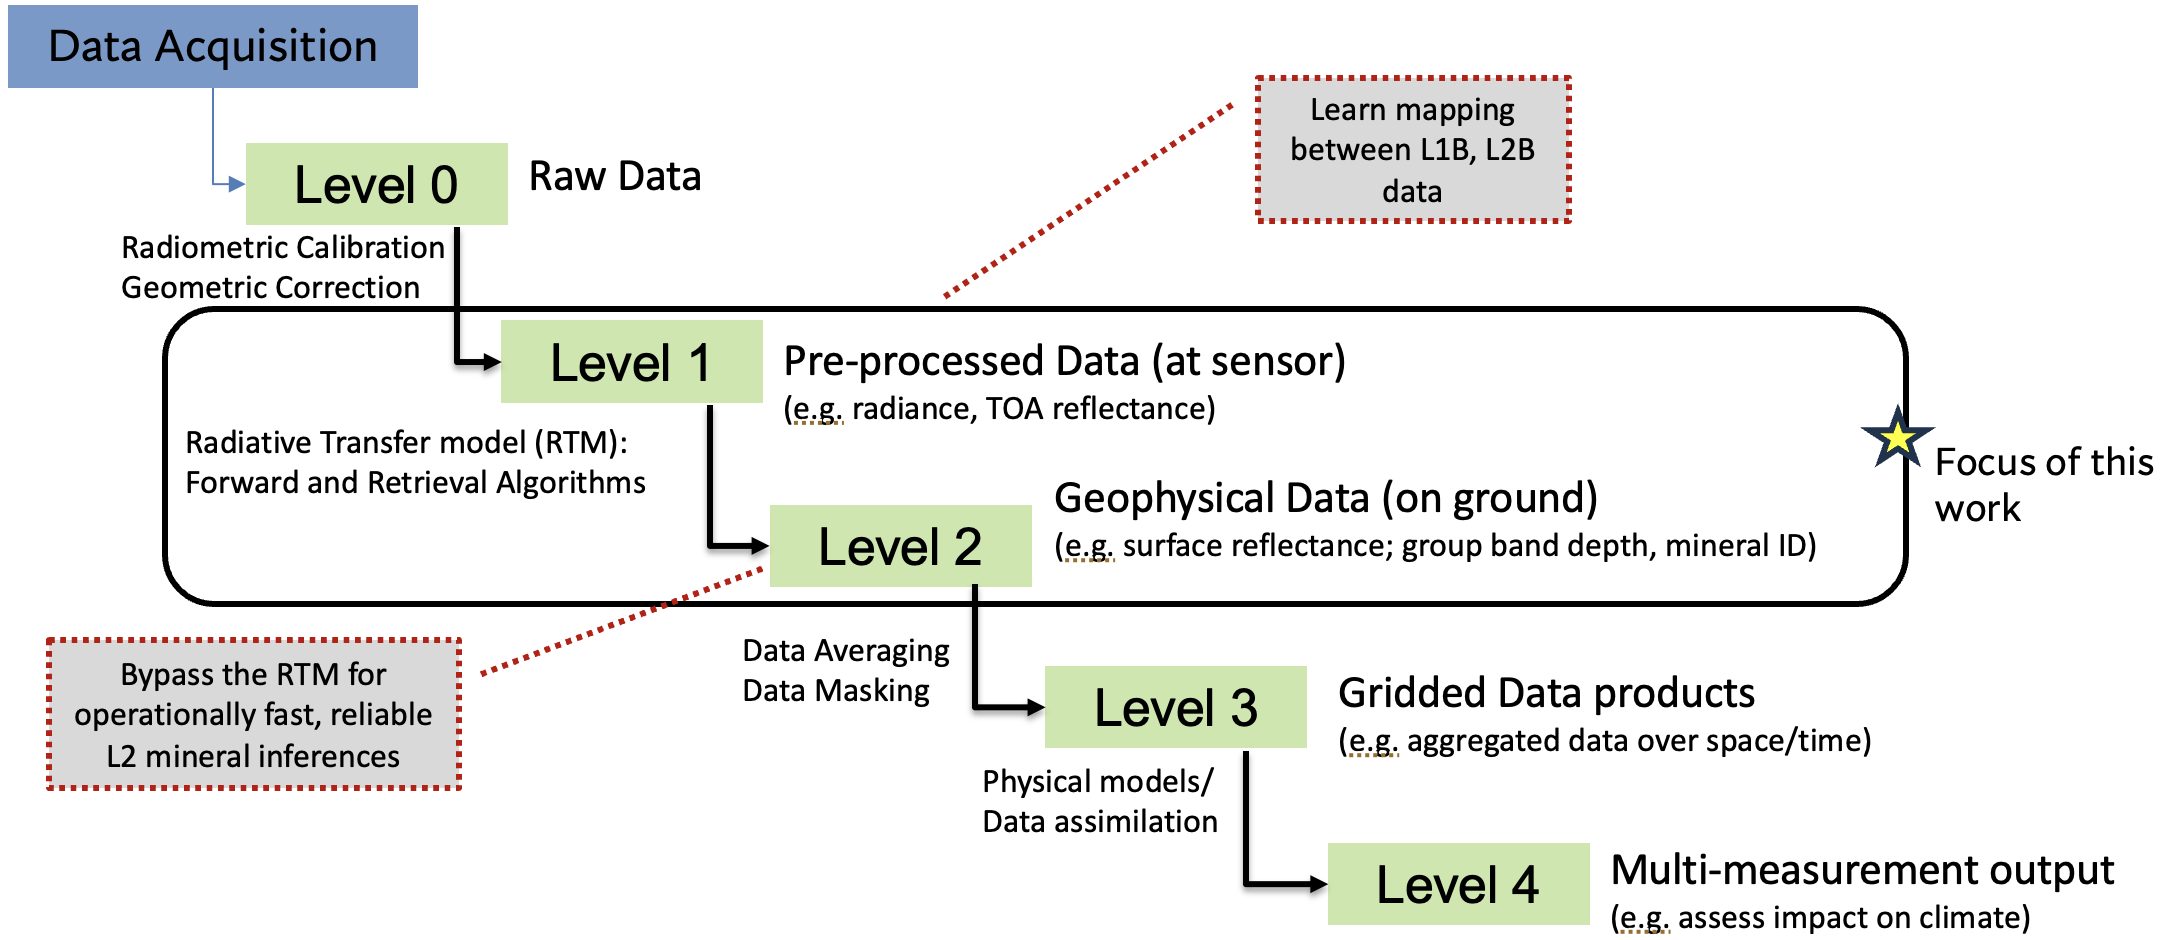
\includegraphics[width=\textwidth]{Data_level_depiction.png}
\caption{Standard SDS processing chain overlayed with the RTM-bypass idea.}
\label{fig:data_levels}
\end{figure}

\subsection{Problem statement and contributions}
\label{subsec:contributions}

For hyperspectral mineral classification, there is a need for scalable, reliable, and efficient methods that produce mineralogical products with latency and cost compatible with operational or onboard deployment needs, generalize across geographic regions and sensor platforms, provide interpretable evidence that learned representations are physically meaningful, and capture invariant mineral structures despite varying observing and atmospheric conditions. 
Existing spectral transformer architectures do not address these requirements simultaneously. 
Most operate on atmospherically corrected reflectance, few offer per-band interpretability, and none explicitly encode invariance to atmospheric perturbation.

This paper makes the following contributions toward filling that gap:
\begin{enumerate}
  \item \textbf{Post-hoc direct retrieval for mineral classification (RTM bypass):} A cross-attention transformer that maps L1B TOA reflectance to a probabilistic distribution over 95 mineral classes (softmax; top-1 and top-3 reported) in a single forward pass, with $O(H \times L)$ complexity linear in the number of spectral bands. Unlike RTM-trained direct retrievals (e.g., \cite{Keely2025ConditionalDiffusionCO2,Li2022NO2NN}), the model is trained on operational L1B/L2B pairs from the EMIT Science Data System and requires no radiative transfer model in either training or inference --- hence the ``RTM bypass'' shorthand used throughout. The compact model ($<$457K parameters) enables millisecond-scale inference, opening pathways to real-time detection of transient phenomena, autonomous revisit prioritization, and onboard processing for bandwidth-constrained missions.
  \item \textbf{Spectroscopic interpretability:} Per-band, per-head attention weights ($\mathbf{A}_h$) validated against known diagnostic absorption features within $\pm$20~nm of literature values, providing physically explainable classification decisions.
  \item \textbf{Physics-informed spectral priors:} An attention bias $\bm{\beta}_h$ based on USGS reference spectra that injects domain knowledge without altering the architecture. This steers attention toward spectrally diagnostic bands while allowing the model to learn from data, and it provides a testbed for evaluating the impact of different priors on performance and interpretability.
  \item \textbf{Statistical-invariance regularization for atmospheric robustness:} A LUSI-inspired consistency loss that penalizes prediction changes under physically motivated, label-preserving perturbations of the input spectrum (broadband brightness scaling and conservative spectral-slope changes). The empirical consequence is improved cross-region generalization at pixel scale.
  \item \textbf{Sensor-agnostic design:} The new approach is not tied to a specific instrument or application domain.
  Cross-scene generalization across geographic regions (Africa/Middle East to southwestern US) is demonstrated, and the architecture is directly applicable to other imaging spectrometer missions and spectral classification problems..
\end{enumerate}

%% ====================================================================
%% 2. BACKGROUND
%% ====================================================================
\section{Background}
\label{sec:background}

Optical remote sensing operates in the visible (0.4--0.7~$\mu$m), near infrared (0.7--1.0~$\mu$m), and short-wave infrared (1.0--2.5~$\mu$m) regions, where reflected solar radiation dominates. 
This spectral range is optimal for mineral identification. 
The sun provides a bright, broadband, stable illumination source, the atmosphere is reasonably transparent, and minerals exhibit rich diagnostic absorption features.

\subsection{The remote sensing data processing chain}

The standard remote sensing science data processing chain, with some perturbations across missions, transforms raw sensor data through hierarchical levels:
\begin{itemize}
  \item \textbf{Level 0:} Raw data from the instrument.
  \item \textbf{Level 1:} Radiometrically calibrated and geometrically corrected data. Level~1B provides at-sensor radiance (often converted to TOA reflectance) \cite{emit_l1b_atbd}.
  \item \textbf{Level 2:} Derived geophysical parameters, including atmospheric correction to surface reflectance (L2A) \cite{emit_l2a_atbd} and mineral identification via Tetracorder (L2B) \cite{emit_l2b_atbd}.
  \item \textbf{Level 3/4:} Gridded and multi-measurement products \cite{emit_l3_atbd}.
\end{itemize}

The transition from Level~1 to Level~2 is the critical bottleneck.
It requires radiative transfer modeling to remove atmospheric effects, followed by spectral matching against reference libraries.

\subsection{Approaches to accelerating retrieval}
\label{sec:rtm_emulation}

Physics-based RTMs such as MODTRAN simulate the propagation of electromagnetic radiation through the atmosphere. 
Operational systems have pivoted toward emulation, constructing statistical or machine learning surrogates that approximate the RTM forward model at a fraction of the computational cost, achieving acceleration factors of $10^2$ to $10^6$.

EMIT's ISOFIT retrieval was originally designed to call the MODTRAN radiative transfer model directly at each OE iteration. 
The flagship emulation example is \textbf{sRTMnet} \cite{brodrick2021, emit_l2a_atbd}, a neural network trained on MODTRAN outputs that replaced these direct RTM calls in the operational pipeline, achieving $>3{,}000\times$ speedup with sub-percent relative error in radiance predictions \cite{brodrick2021} --- well within EMIT's 3.1--6.0\% radiometric uncertainty (Table~\ref{tab:emit_specs}). 
Crucially, sRTMnet \emph{accelerates} the existing pipeline; 
ISOFIT still performs iterative OE to retrieve atmospheric state and surface reflectance, and Tetracorder still performs mineral identification on the corrected surface reflectance. 
The same processing steps occur; only the forward model computation is faster.

A distinction among acceleration methods is whether they operate \emph{in-line} (embedded within the operational pipeline, accelerating existing steps) or \emph{post-hoc} (trained on already-processed data products). Each approach represents a different choice about \emph{what is learned} and \emph{what is bypassed}:
\begin{itemize}
  \item \textbf{Forward emulator}: learns $F_{\theta}(\mathbf{x}) \approx F(\mathbf{x})$, a fast surrogate for the radiative transfer forward model. Bypasses only the expensive RTM call. The retrieval itself (the inverse solve) is still iterative, and $F_{\theta}$ is invoked many times per pixel within the loop.
  \item \textbf{Retrieval emulator (direct retrieval)}: learns $g_{\theta}(\mathbf{y}) \approx \hat{\mathbf{x}}_{\text{retrieval}}$, a single-pass mapping from measurement to retrieved state. Bypasses the entire retrieval processor --- the inverse solve, including any iteration --- at inference. The forward model is invoked only offline, to synthesize $(\mathbf{x}, \mathbf{y})$ training pairs.
  \item \textbf{Post-hoc direct retrieval / RTM bypass} (this work): learns $h_{\theta}(\mathbf{y}) \approx \text{mineral~ID}$ from operational SDS outputs. Bypasses the RTM and the entire retrieval $+$ spectral-matching chain. Crucially, no RTM is invoked even at training time --- training pairs come from the operational SDS pipeline rather than from RTM-synthesized data.
\end{itemize}

\begin{table}[!htbp]
\centering
\small
\caption{Spectrum of approaches for accelerating spectral remote-sensing retrieval. Speed is not directly comparable across rows because baselines differ.}
\label{tab:emulation_spectrum}
\begin{tabular}{p{0.28\textwidth}p{0.24\textwidth}p{0.24\textwidth}p{0.12\textwidth}}
\hline
\rowcolor[gray]{0.85}
\textbf{Approach, examples} & \textbf{RTM role} & \textbf{Acceleration target} & \textbf{Speedup} \\
\hline
Forward emulator\newline \emph{e.g., sRTMnet \cite{brodrick2021}, GP/OCO-2 \cite{lamminpaa2025}, FastMAPOL \cite{gao2023}} & Surrogate for RTM forward model, typically used in-line within retrieval or LUT generation & Per-call or per-iteration RTM evaluation within a retrieval workflow & $10^2$--$10^4\times$ \\
\hline
Retrieval emulator / direct learned retrieval\newline \emph{e.g., Keely et al.~\cite{Keely2025ConditionalDiffusionCO2} probabilistic diffusion; Li et al.~\cite{Li2022NO2NN} deterministic NN} & RTM and/or operational retrieval used offline for synthetic training data or labels; not invoked at inference & End-to-end measurement $\to$ retrieved geophysical state or posterior, replacing much of the conventional retrieval processor & $10^1$--$10^5\times$ \\
\hline
Post-hoc direct retrieval surrogate\newline \emph{this work; categorical transformer over 95 mineral classes} & RTM not invoked by proposed model; physical/retrieval assumptions inherited through operational SDS labels & End-to-end L1B/TOA spectrum $\to$ mineral-class posterior & $10^4$--$10^6\times$ \\
\hline
\end{tabular}
\end{table}

The method in this paper is fundamentally post-hoc.
It trains on paired L1B TOA reflectance and L2B mineral identification products that have been fully processed through the EMIT SDS.
The model learns the mapping from L1B TOA reflectance to L2B mineral class and applies it to new L1B observations without re-invoking any component of the SDS.

\subsection{Approaches to physics-informed retrieval}
\label{subsec:physics_informed_approaches}

Beyond pure speed, recent work in remote-sensing machine learning the value of encoding physical knowledge directly into model architectures and training objectives. 
\emph{Physics-informed neural networks} (PINNs) embed governing equations or boundary conditions as penalty terms in the loss function~\cite{raissi2019pinn}.
The broader \emph{theory-guided data science} paradigm~\cite{karpatne2017tgds} extends this to incorporating domain knowledge as priors, constraints, or feature engineering. 
In hyperspectral retrieval, two physics-injection mechanisms are relevant to this work: priors derived from reference spectral libraries that bias attention toward mineralogically informative wavelengths, and invariance constraints that encode physical symmetries the predicted label should ignore.

The closest hyperspectral analogue to the spectral-prior mechanism developed here is Wang et al.~\cite{wang2021attention_pca_guided}, who use PCA-guided self-supervised feature extraction within an attention-based spatial--spectral network for hyperspectral change detection. 
The construction in this paper differs in two ways: PCA is computed on an \emph{external} reference library (USGS Spectral Library~\cite{kokaly2017usgs}), and the resulting absolute loadings initialize an additive \emph{pre-softmax attention bias} rather than a self-supervised auxiliary target. 
This produces a soft, trainable initialization that anchors selected attention heads to mineralogically meaningful wavelengths while allowing supervised training on TOA reflectance to refine or override the prior (Section~\ref{sec:pca_priors}).

For invariance, this work draws on Vapnik and Izmailov's complete statistical theory of learning~\cite{vapnik2020}, which formalizes domain knowledge as \emph{predicates} and \emph{statistical invariants} that restrict the admissible function class. 
Direct applications of LUSI to remote sensing are sparse; this paper implements a transformation-based approximation suited to neural training, borrowing the teacher--student consistency-loss pattern from knowledge distillation~\cite{hinton2015distilling}. 
The two mechanisms are complementary. 
PCA priors guide \emph{where} attention starts, the invariance loss constrains \emph{what perturbations} should not change the predicted mineral identity (Section~\ref{sec:lusi}).
To the authors' knowledge, no prior work has combined both for hyperspectral mineral classification.

%% ====================================================================
%% 3. EMIT INSTRUMENT AND DATA
%% ====================================================================
\section{EMIT: Instrument and data structures}
\label{sec:emit}

The EMIT instrument is a Dyson imaging spectrometer utilizing six optical elements to achieve high signal-to-noise ratios and spectral uniformity exceeding 98\% \cite{thompson_emit_2024}.
Each EMIT granule contains a three-dimensional hyperspectral data cube structured as $1280 \times 1242$ spatial pixels across 285 spectral bands, stored as NetCDF files \cite{emit_l1b_atbd}.
This study leverages approximately 396 granules across Africa and the Middle East (Figure~\ref{fig:africa_collection}), an intentionally small sample.
Training and validation pixels are sampled from this set of granules.

\begin{wrapfigure}{r}{0.60\textwidth}
\centering
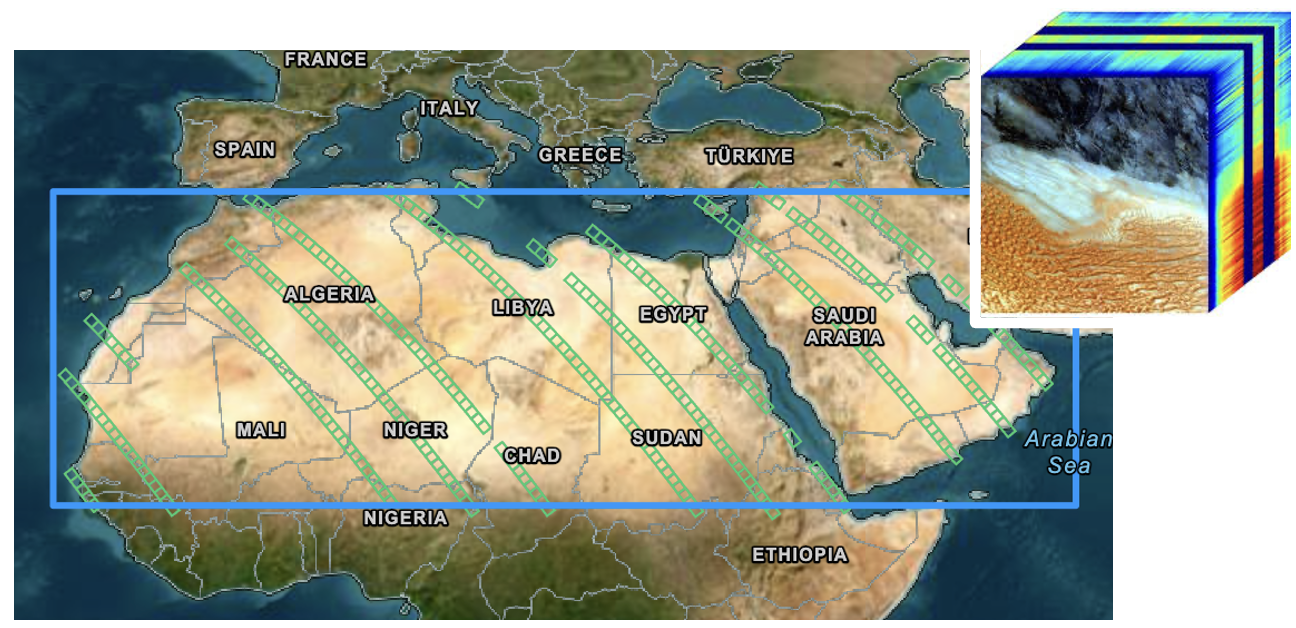
\includegraphics[width=0.60\textwidth]{Africa-collection.png}
\caption{A small representative set of initial EMIT data products are generated from the mission's SDS. 
Green tracks show the $\sim$396 granules across Africa and the Middle East used for training in this study.}
\label{fig:africa_collection}
\end{wrapfigure}

An additional 52 granules from the Southwest US are used for disjoint geographical model testing. 

\subsection{Radiance and TOA reflectance}
\label{sec:radiance_toa}

The EMIT L1B product provides calibrated at-sensor spectral radiance $R_j^M$ in units of $\mu$W\,nm$^{-1}$\,cm$^{-2}$\,sr$^{-1}$.
For mineral classification, this is converted to dimensionless TOA reflectance via $\rho_{\text{toa},j} = \pi R_j^M / (F_j \cos\theta)$, where $R_j^M$ is the measured radiance at band $j$, $F_j$ is the extraterrestrial solar spectral irradiance, and $\theta$ is the solar zenith angle.
Unlike surface reflectance (L2A), TOA reflectance conflates the surface signal with atmospheric path radiance and transmittance, so the model must learn to classify minerals without these effects being removed.

\subsection{Mineral grouping and spectral libraries}

EMIT's mineral identification uses a grouping matrix containing 293 reference spectra organized into Group~1 ($Q_1 = 95$ classes, primarily iron oxides, pyroxenes, and feldspars) and Group~2 ($Q_2 = 199$ classes, primarily clays, carbonates, and sulfates).
Reference spectra are drawn from the USGS Spectral Library \cite{kokaly2017usgs}, and mineral identification is performed using the Tetracorder expert system \cite{emit_l2b_atbd, clark2003tetracorder}.
The mission specifically targets ten dust-source minerals selected for their climate-forcing relevance: hematite, goethite, calcite, dolomite, gypsum, illite+muscovite, kaolinite, montmorillonite, chlorite, and vermiculite \cite{emit_factsheet, emit_l3_atbd}.
Of these, only hematite and goethite are classified as Group~1; the remaining eight clay/carbonate/sulfate species are assigned to Group~2.
This split is consistent with the spectroscopic and climate-forcing rationale: hematite and goethite produce the strongest radiative forcing uncertainty in dust models (Section~\ref{sec:intro}) and exhibit the diagnostic Fe$^{3+}$ features summarized in Table~\ref{tab:fe_diagnostics}, motivating Group~1 as the primary classification target.
This work will focus on Group~1 mineral classification; Group~2 classification parallels this approach.

A primary challenge is spectral confusion between mineral species.
The hematite--goethite discrimination is particularly demanding because both minerals exhibit similar Fe$^{3+}$ electronic absorption structure in the VNIR, including overlapping absorptions near 0.86--0.92~$\mu$m \cite{clark1999,sherman1985}.
They differ primarily in the detailed band shape and position of diagnostic visible features, including derivative-spectrum minima near $\sim$480~nm for goethite and $\sim$535~nm for hematite \cite{Jiang2014AlGoethite}.

In plain terms: electrons in an atom occupy specific energy levels and can only absorb light whose energy matches a level-to-level gap exactly. \emph{Crystal-field} transitions are jumps within a single iron atom, between $d$-orbital levels that are slightly split by the surrounding oxygen ligands --- for Fe$^{3+}$ in iron oxides, these produce the weaker absorption features near $\sim$670~nm and in the NIR. \emph{Charge-transfer} transitions are stronger jumps where an electron moves from an oxygen atom \emph{to} an iron atom; they peak in the ultraviolet, but the absorption tail extending into the visible yields the steep edge that produces the diagnostic $\sim$480~nm (goethite) and $\sim$535~nm (hematite) features. Table~\ref{tab:fe_diagnostics} summarizes the canonical band assignments used in the per-head attention analysis (Section~\ref{sec:ablation}). See \cite{burns1993,clark1999,sherman1985,Jiang2014AlGoethite} for comprehensive treatments.

\begin{table}[H]
\centering
\small
\caption{Canonical Fe$^{3+}$ diagnostic absorption bands. The visible bands (~535/~480~nm) are charge-transfer features (responsible for the minerals' colors); the longer-wavelength bands are crystal-field features, with goethite's NIR feature shifted to $\sim$920~nm versus hematite's $\sim$860~nm --- the key discriminator between the two minerals.}
\label{tab:fe_diagnostics}
\begin{tabular}{p{0.10\textwidth}p{0.20\textwidth}p{0.55\textwidth}}
\hline
\rowcolor[gray]{0.85}
\textbf{Mineral} & \textbf{Diagnostic bands (nm)} & \textbf{Physical origin} \\
\hline
Hematite & $\sim$535 & Charge-transfer region; absorbs green $\to$ mineral looks red. \\
\hline
Hematite & $\sim$670, $\sim$860 & Crystal-field region; 860~nm is the main NIR fingerprint. \\
\hline
Goethite & $\sim$480 & Charge-transfer region; absorbs blue $\to$ mineral looks rust-yellow. \\
\hline
Goethite & $\sim$670, $\sim$920 & Crystal-field region; the 920~nm shift (vs hematite's 860~nm) is what tells the two minerals apart. \\
\hline
\end{tabular}
\end{table}

%% ====================================================================
%% 4. RELATED WORK: SPECTRAL TRANSFORMERS
%% ====================================================================
\section{Related work: Spectral transformers for hyperspectral analysis}
\label{sec:related}

Shallow classifiers (SVMs, random forests) paired with dimensionality reduction (PCA, LDA) formed the standard HSI pipeline for decades.
Deep learning brought 1D, 2D, and 3D CNNs that model local spatial-spectral correlations \cite{hong2021spectralformer}, but CNNs are fundamentally limited by localized receptive fields.
In mineral analysis, discriminative absorption features are distributed across distant wavelengths (e.g., Fe$^{3+}$ charge transfer at $\sim$535~nm and crystal field transitions at $\sim$860~nm).
The Transformer architecture \cite{vaswani2017attention} provided an alternative via multi-head self-attention:
\begin{equation}
\text{Attention}(\mathbf{Q}, \mathbf{K}, \mathbf{V}) = \text{Softmax}\!\left(\frac{\mathbf{Q}\mathbf{K}^T}{\sqrt{d_k}}\right)\mathbf{V},
\label{eq:self_attention}
\end{equation}
where $d_k$ is the dimension of the key vectors $\mathbf{K} \in \R^{n \times d_k}$. 
However, the $\mathbf{Q}\mathbf{K}^T$ product gives self-attention $O(L^2)$ complexity, motivating the pursuit of efficient alternatives.

\subsection{Architectural and methodological foundations}
\label{sec:arch_inspirations}

Three works directly inspired the design presented here.
Table~\ref{tab:arch_inspirations} maps each foundational concept to its source.

\paragraph{Shape-aware tokenization: spectral derivatives}
Derivative analysis is commonly used in hyperspectral spectroscopy to emphasize local spectral structure and extract subtle band-shape information from spectrally continuous measurements. 
Tsai and Philpot \cite{tsai1998derivative} describe both Savitzky--Golay convolutional derivatives and finite divided-difference approximations along the wavelength axis. 
This work adopts the latter idea at the tokenization stage.
Each band is encoded with its raw reflectance together with first and second finite differences along $\lambda$, producing a shape-aware per-band feature vector before cross-attention evaluates global spectral context.

\paragraph{Perceiver: Cross-attention}
Jaegle et al.\ \cite{jaegle2021perceiver} introduced the Perceiver architecture, which uses a fixed-size set of learned latent queries to cross-attend to a much larger input array. 
This asymmetric attention pattern avoids computing self-attention over all $L$ input tokens, reducing the input-attention cost from $O(L^2)$ to $O(M \times L)$ for $M \ll L$ latent queries. 
We adopt this Perceiver-style cross-attention principle for spectral pooling. 

\paragraph{SpecTf: Per-pixel spectral modeling}
SpecTf \cite{lee2025spectf} demonstrated that treating imaging-spectrometer measurements as 1-D spectral sequences can support accurate per-pixel cloud detection on EMIT without spatial or temporal context.
The model significantly outperformed the operational EMIT cloud-mask baseline.
Its attention weights emphasized physically meaningful atmospheric absorption regions, motivating the per-pixel spectral-only modeling strategy adopted here.

\begin{table}[!htbp]
\centering
\small
\caption{Architectural lineage: mapping foundational concepts to this work.}
\label{tab:arch_inspirations}
\begin{tabular}{p{0.70\textwidth}p{0.22\textwidth}}
\hline
\rowcolor[gray]{0.85}
\textbf{This Work} & \textbf{Source} \\
\hline
1.\ Shape-aware tokenization via spectral derivatives & Derivative analysis \cite{tsai1998derivative} \\
\hline
2.\ Asymmetric cross-attention with $H$ learned queries ($\mathbf{q}_h$) & Perceiver \cite{jaegle2021perceiver} \\
\hline
3.\ Cross-attention sequence pooling ($\mathbf{z}_{\text{cat}}$) & Perceiver \cite{jaegle2021perceiver} \\
\hline
4.\ Per-pixel spectral classification (no spatial context) & SpecTf \cite{lee2025spectf} \\
\hline
5.\ Per-head attention validation against mineral diagnostics & SpecTf \cite{lee2025spectf} \\
\hline
\end{tabular}
\end{table}

The architectures reviewed above all assume atmospherically corrected input or target atmospheric phenomena rather than surface mineralogy. 
To the authors' knowledge, no prior spectral transformer attempts HSI mineral classification directly from L1B TOA reflectance, with the speed and reliability enabled by the RTM bypass and the physics-informed components described in this paper.
The architecture described in the next section addresses the implementation.

%% ====================================================================
%% 5. ARCHITECTURE
%% ====================================================================
\section{Architecture}
\label{sec:architecture}

The proposed architecture is a cross-attention transformer designed specifically for per-pixel spectral classification from hyperspectral TOA reflectance. 
It departs from conventional self-attention transformers (which were designed for natural language and images) in three substantive ways: shape-aware tokenization encodes each band with its raw reflectance plus first and second finite differences along $\lambda$ \cite{tsai1998derivative}; the queries are learned rather than derived from the input, reducing attention complexity from $O(L^2)$ to $O(H \times L)$; and the attention bias provides a physics-injection interface for USGS-derived spectral priors (Section~\ref{sec:physics}) while a Vapnik-style consistency regularizer (Section~\ref{sec:lusi}) accommodates statistical invariants drawn from physically motivated perturbations of TOA reflectance.
The remainder of this section walks through preprocessing, tokenization, attention pooling, classification head, and optimization, and summarizes the parameter budget; Figure~\ref{fig:architecture} provides the full pipeline overview.

\subsection{Data preprocessing and normalization}
\label{sec:preprocessing}

All operations in this subsection are performed in the original $L$-dimensional reflectance space; no embedding into a higher-dimensional latent space happens until tokenization (Section~\ref{sec:tokenization}).
The training data consists of $N = 1{,}260{,}203$ class-balanced pixels drawn from EMIT L1B TOA reflectance over Africa and the Middle East (396 granules), split 90/10 into training and validation with a fixed random seed.
Each pixel has $L = 285$ spectral bands and a Group~1 mineral class label from the EMIT SDS pipeline.

The raw Tetracorder-assigned Group~1 distribution is highly imbalanced (Figure~\ref{fig:g1_hist}), spanning several orders of magnitude.
The top nine populated classes are all iron-bearing minerals, consistent with EMIT's mission focus on iron-oxide-rich arid dust source regions \cite{emit_factsheet}; three of the 95 expected IDs are entirely absent in the study region (IDs 1, 72, 74), so 92 of 95 classes are populated.
A stratified per-class cap of 7{,}500 pixels prevents the model from collapsing onto the dominant classes; 20 of the 92 populated classes nonetheless fall short of the cap (one to 1{,}328 pixels), reflecting the natural rarity of some minerals in the study region.

\begin{wrapfigure}{r}{0.7\textwidth}
\centering
\vspace{-1em}
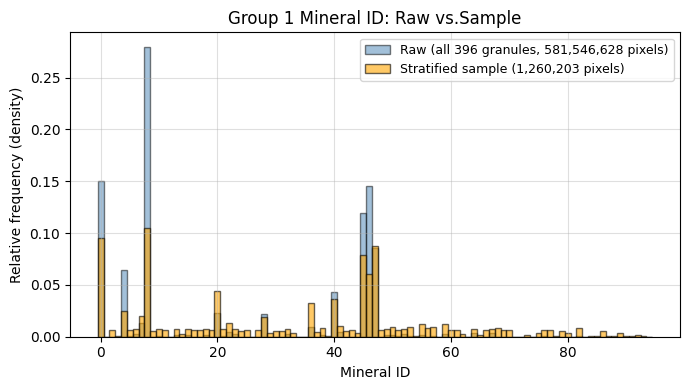
\includegraphics[width=\linewidth]{G1_orig_samphist.png}
\caption{Group~1 mineral ID distribution before and after stratified sampling. The stratified sample with a 7{,}500 per-class cap flattens this distribution so every populated class is represented.}
\label{fig:g1_hist}
\vspace{-1em}
\end{wrapfigure}

\paragraph{Label preparation}
Class~0 (Tetracorder unclassified) is filtered, and labels are shifted to $0\ldots 94$ for zero-indexed cross-entropy.

\paragraph{Robust normalization}
Per-band robust z-score normalization (per-band median and interquartile range, Figure~\ref{fig:architecture}) is computed on the training split and re-applied without re-fitting at validation and inference. Median--IQR is preferred to mean--standard deviation because TOA distributions are heavy-tailed (atmospheric path radiance, sub-pixel cloud, shadow). A trainable per-band affine $\hat{w}'_j = \gamma_j \hat{w}_j + \delta_j$ ($\gamma_j$ initialized to $1$, $\delta_j$ to $0$) follows the normalization, allowing the model to recover task-useful per-band scaling after magnitudes are stabilized.

\begin{figure}[!htbp]
\centering
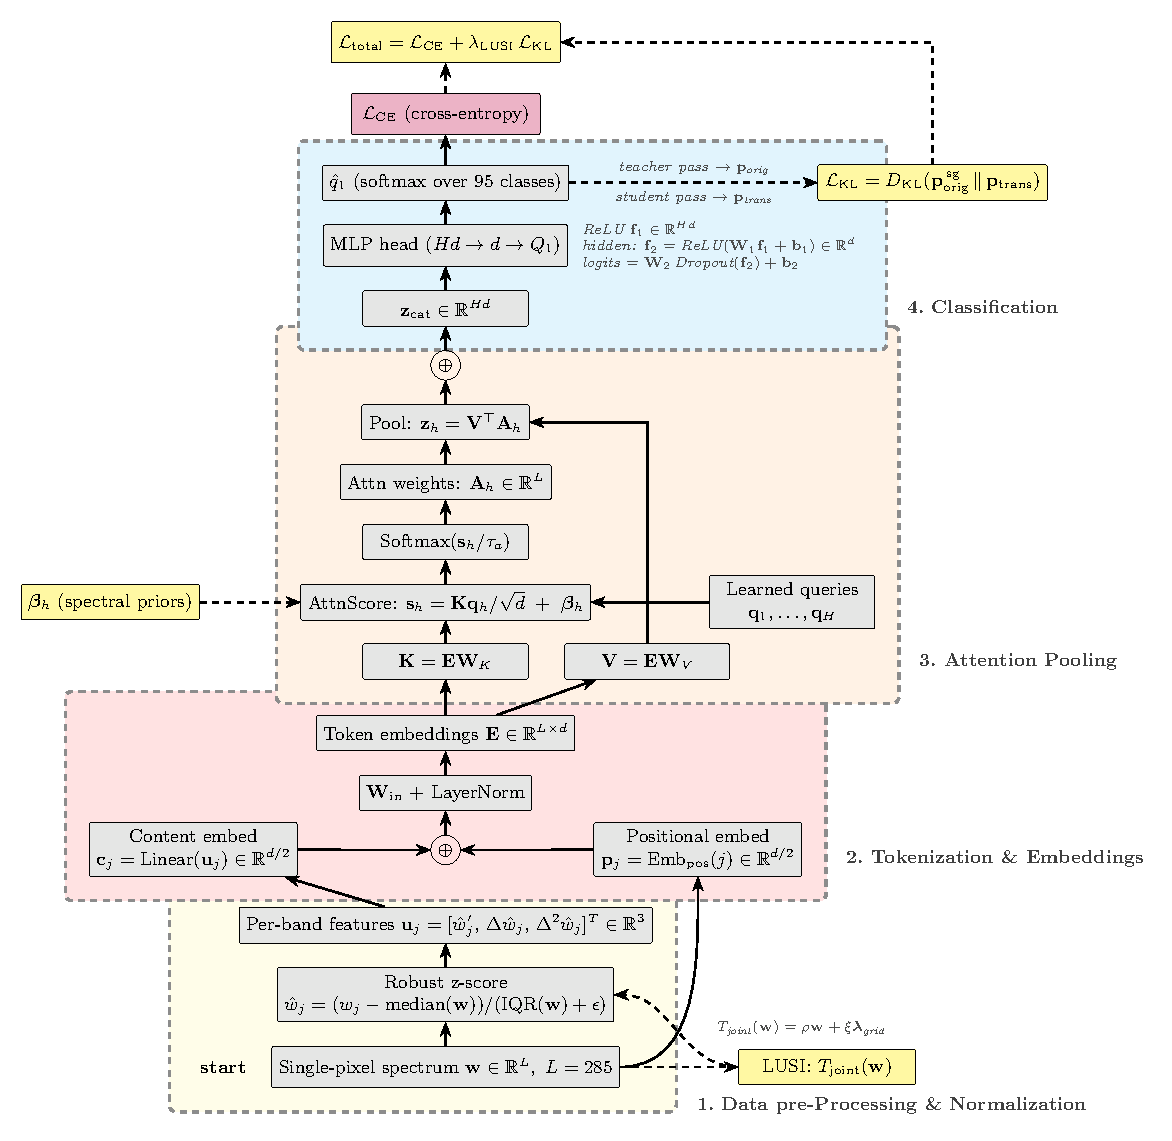
\includegraphics[width=\textwidth]{architecture.pdf}
\caption{End-to-end architecture overview. The forward pass is partitioned into four shaded regions that align with Sections~\ref{sec:preprocessing} (data preprocessing and normalization), \ref{sec:tokenization} (tokenization and embedding), \ref{sec:attn_pooling} (attention pooling), and~\ref{sec:classification} (classification head). 
Optional physics-informed components (yellow boxes, dashed lines). the spectral-priors attention bias and the LUSI consistency branch, can be toggled independently.}
\label{fig:architecture}
\end{figure}


\paragraph{Spectral derivatives.}
Finite-difference first and second derivatives along the wavelength axis encode local absorption-feature morphology, producing a per-band feature vector $\mathbf{u}_j = [\hat{w}'_j, \Delta\hat{w}_j, \Delta^2\hat{w}_j]^T \in \R^3$ that captures absorption depth, asymmetry, and width (Figure~\ref{fig:architecture}).

\subsection{Tokenization and embedding}
\label{sec:tokenization}

Each spectral band corresponds to one token; a pixel's $L = 285$-band spectrum becomes a sequence of 285 tokens. The per-band feature vector $\mathbf{u}_j$ is split into a content embedding $\mathbf{c}_j \in \R^{d/2}$ via a learned linear layer and a learned positional embedding $\mathbf{p}_j \in \R^{d/2}$, then fused into a single token embedding $\mathbf{e}_j \in \R^d$ via a linear mixing layer with LayerNorm (Figure~\ref{fig:architecture}). The mixing layer ensures that downstream attention sees content and position as a single coherent representation rather than two disjoint blocks. The embedding dimension $d = 192$ is split evenly ($d/2 = 96$ each), in the range of compact transformer precedents (e.g.\ DeiT-Tiny, SpecTf~\cite{lee2025spectf}); a sweep over $d$ for an accuracy optimum is left as future work.

\subsection{Attention pooling}
\label{sec:attn_pooling}

The 285-token sequence is reduced to a single summary vector via \emph{cross-attention with learned queries}: each of $H$ query vectors $\mathbf{q}_h \in \R^d$ (one per head) is compared against per-band keys $\mathbf{K} = \mathbf{E}\mathbf{W}_K$ to produce attention weights, which then pool per-band values $\mathbf{V} = \mathbf{E}\mathbf{W}_V$, with $\mathbf{W}_K, \mathbf{W}_V \in \R^{d \times d}$ and $\mathbf{E} = [\mathbf{e}_1,\ldots,\mathbf{e}_L]^T$ (Figure~\ref{fig:architecture}). Treating the queries as $H$ independent model parameters --- rather than as projections of the sequence itself --- reduces complexity from $O(L^2)$ to $O(H L)$ and makes the resulting attention weights directly interpretable as per-band importance scores.

The $H$ queries $\mathbf{q}_h$ are initialized from $\mathcal{N}(\mathbf{0}, \mathbf{I})$ and updated by gradient descent on the classification loss; each can be interpreted as a learned spectral ``question'' the model poses to the input. The per-head attention scores and weights are
\begin{equation}
\mathbf{s}_h = \frac{\mathbf{K}\mathbf{q}_h}{\sqrt{d}} + \bm{\beta}_h \in \R^L, \qquad \mathbf{A}_h = \text{Softmax}\!\left(\frac{\mathbf{s}_h}{\tau_a}\right) \in \R^L,
\label{eq:attn_score}
\end{equation}
where the $\sqrt{d}$ scaling prevents softmax saturation and the temperature $\tau_a = 0.9$ keeps the softmax peaked but multi-band ($\tau_a$ sensitivity was not ablated and is left for future work). The pooled head vector $\mathbf{z}_h = \mathbf{V}^T \mathbf{A}_h \in \R^d$ and the concatenation $\mathbf{z}_{\text{cat}} = \mathbf{z}_1 \oplus \cdots \oplus \mathbf{z}_H \in \R^{Hd}$ complete the attention block (Figure~\ref{fig:architecture}). The additive bias $\bm{\beta}_h \in \R^L$ is the interface for physics-informed priors (Section~\ref{sec:physics}): when priors are absent, $\bm{\beta}_h$ is held at $\mathbf{0}$ throughout training; when priors are present, $\bm{\beta}_h$ is initialized at the prior values and trainable from epoch~1 (or after a configurable warm-up freeze). The split between $\mathbf{K}$ and $\mathbf{V}$ lets the model decide \emph{where to look} and \emph{what to read} with independent parameters.

\subsection{Classification head}
\label{sec:classification}

The pooled vector $\mathbf{z}_{\text{cat}}$ is mapped to per-class logits by a two-layer feed-forward network with ReLU activations and dropout $p = 0.1$, compressing the $Hd = 1{,}536$-dimensional multi-head representation to $d = 192$ before producing $Q_1 = 95$ class logits (Figure~\ref{fig:architecture}); the predicted mineral ID $\hat{q}_{1}$ is the argmax over those logits. The softmax distribution $\hat{\mathbf{p}}$ over $Q_1 = 95$ classes is a \emph{model} probability rather than a calibrated estimate of real-world class probabilities; we report top-1 and top-3 retrievals as relative measures and treat any frequentist interpretation as requiring separate calibration.

\subsection{Model parameter summary}

The model is compact, with 307{,}373 learnable parameters at $H = 4$ and 456{,}737 at $H = 8$, orders of magnitude smaller than typical vision transformers. These counts depend on $d = 192$, $L = 285$, $Q_1 = 95$, and $c_{in} = 3$.

\subsection{Optimization}
\label{sec:optimization}

The training objective is cross-entropy with label smoothing:
\begin{equation}
\mathcal{L}_{\text{CE}} = -\sum_{c=1}^{Q_1} \tilde{q}_c \log \hat{p}_c, \quad \tilde{q}_c = (1 - \epsilon_{\text{ls}}) q_c + \frac{\epsilon_{\text{ls}}}{Q_1},
\label{eq:ce_loss}
\end{equation}
where $q_c \in \{0,1\}$ is the one-hot ground-truth label, $\hat{p}_c$ is the predicted class probability, and $\epsilon_{\text{ls}} = 0.05$. Label smoothing prevents the model from driving the correct-class logit to $+\infty$ and provides regularization given the noise in Tetracorder labels and the small population of several Group~1 classes \cite{szegedy2016rethinking}.

AdamW \cite{loshchilov2019adamw} is used with two parameter groups: a main group containing every learnable parameter except $\bm{\beta}_h$ (weight decay $3 \times 10^{-3}$), and a separate group for $\bm{\beta}_h$ with weight decay $= 0$ (active only when priors are used). A cosine annealing schedule with linear warmup over the first 5\% of training steps controls the learning rate between $\eta_{\max} = 5 \times 10^{-4}$ and $\eta_{\min} = 0.1\,\eta_{\max}$.

\subsection{Transformer-only results}
\label{sec:trans_only_results}

The architecture of Section~\ref{sec:architecture} is first evaluated with $\bm{\beta}_h = \mathbf{0}$ (frozen) and no LUSI, to establish the baseline against which the physics-informed (Section~\ref{sec:physics}) and LUSI (Section~\ref{sec:lusi}) variants are compared in Section~\ref{sec:ablation}.
All wall-clock timings throughout this work were measured on a single Apple~M4~Max laptop with PyTorch's MPS backend, using a fixed random seed and identical data pipeline across configurations.

\begin{table}[!htbp]
\centering
\small
\caption{Transformer-only baseline on the held-out validation split. Both configurations use a trainable per-head attention bias $\bm{\beta}_h$ initialized at zero, which Section~\ref{sec:ablation} establishes as the parameter-matched reference for the prior-bearing configurations.}
\label{tab:trans_only_results}
\begin{tabular}{p{0.20\textwidth}p{0.10\textwidth}p{0.15\textwidth}p{0.15\textwidth}p{0.18\textwidth}}
\hline
\rowcolor[gray]{0.85}
\textbf{Configuration} & \textbf{\#Heads} & \textbf{Top-1 Acc.} & \textbf{Top-3 Acc.} & \textbf{Train + Val Time (min)} \\
\hline
Transformer & 4 & 0.789 & 0.961 & 119 \\
\hline
Transformer & 8 & 0.819 & 0.970 & 134 \\
\hline
\end{tabular}
\end{table}

Doubling heads from 4 to 8 yields $+3.0$~pp top-1 and $+0.9$~pp top-3 at a $\sim$13\% wall-clock cost.
At the class level, the two illustrative iron oxides perform well on the held-out split:
hematite reaches precision/recall/F1 of $0.922 / 0.945 / 0.934$ ($N = 729$), goethite $0.877 / 0.957 / 0.915$ ($N = 141$).

\paragraph{Non-attention baseline} A random-forest classifier (500 trees, $\sqrt{L}$ features per split, otherwise default scikit-learn settings) trained on the same Group~1 split reaches top-1 = $0.716$ and top-3 = $0.922$ in $\sim$22~minutes of CPU training. The unguided $H = 4$ transformer above clears this baseline by $7.3$~pp top-1 before any physics priors are applied, isolating the contribution of \emph{learned} band-to-band structure (cross-attention plus value-pathway combinations) over per-band thresholding. The forest also exhibits a wider top-1-to-top-3 spread ($+20.6$~pp vs.\ $+15.1$~pp for Trans~$H = 8$): it knows the answer is in its top three predictions almost as often as the transformer does, but is more uncertain among those three --- the signature of a model that has learned per-band decision rules without learning band-to-band relationships.

\paragraph{Head-averaged attention across the four parameter-matched 4H configurations}
Figure~\ref{fig:trans4_attn} compares head-averaged attention $\bar{\mathbf{A}}^{(c)} = \frac{1}{H}\sum_h \mathbf{A}_h^{(c)} \in \R^{285}$ on hematite (top) and goethite (bottom) at $H = 4$ across the four configurations of Table~\ref{tab:ablation}. Dashed vertical lines mark the literature Fe$^{3+}$ diagnostic wavelengths for each mineral; light gray spans show the H$_2$O atmospheric masks. Because the inputs are TOA reflectance with derivative-aware tokenization, exact coincidence between attention maxima and laboratory absorption centers is not expected; the relevant question is whether attention concentrates in physically plausible neighborhoods, and how the spectroscopic prior reshapes which neighborhoods receive attention mass.

\begin{figure}[!htbp]
\centering
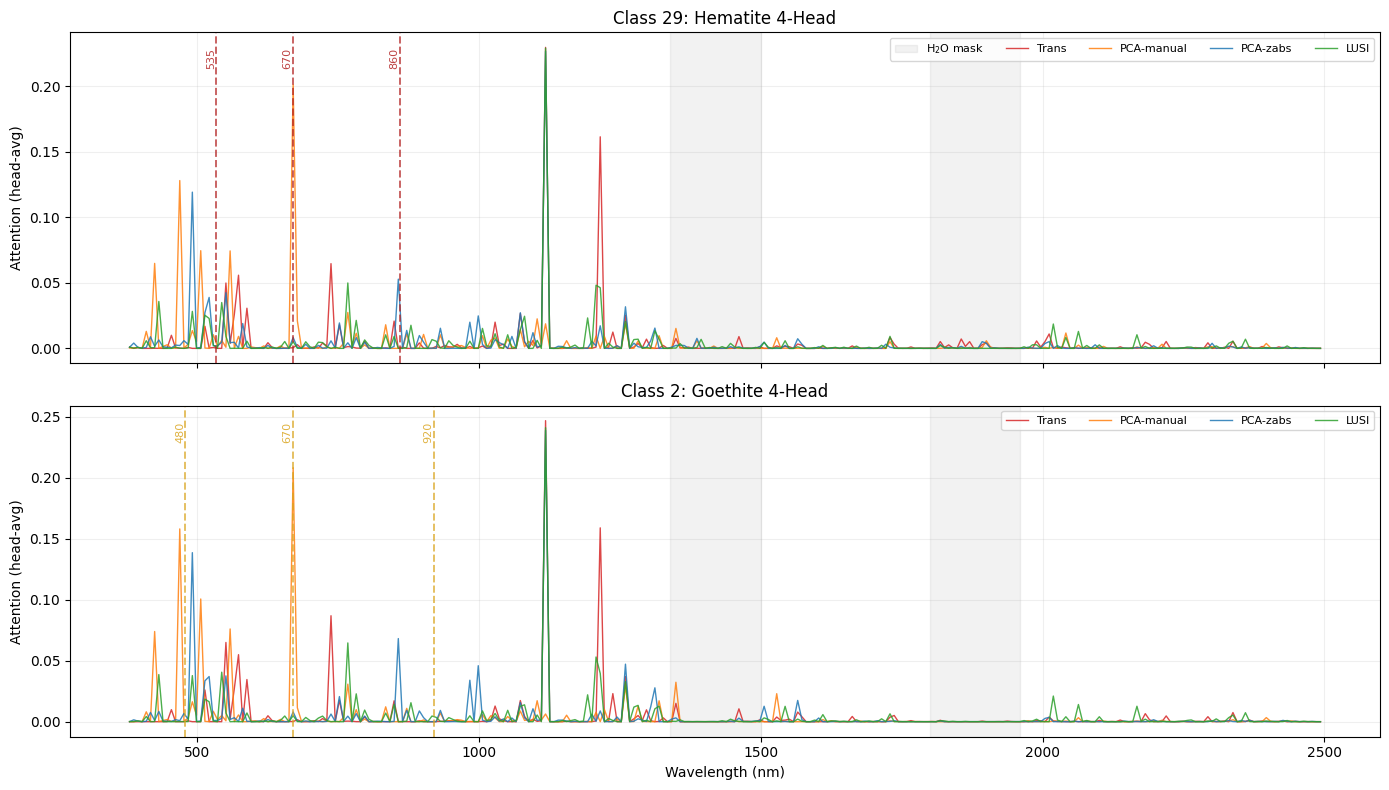
\includegraphics[width=\textwidth]{attention_headavg_compare4h.png}
\caption{Head-averaged class-conditional mean attention weights $\bar{\mathbf{A}}^{(c)} \in \R^{285}$ for hematite (top, class~29) and goethite (bottom, class~2) at $H = 4$, comparing the four parameter-matched configurations of Table~\ref{tab:ablation}: transformer baseline (red), PCA-manual prior (orange), PCA-curated prior (blue), and LUSI-only (green). Vertical dashed lines mark the literature Fe$^{3+}$ charge-transfer and crystal-field diagnostic wavelengths for each mineral (hematite: 535/670/860; goethite: 480/670/920); light gray spans show the H$_2$O atmospheric masks.}
\label{fig:trans4_attn}
\end{figure}

\paragraph{Quantitative validation: Spearman rank correlation against per-mineral absorption depth.}
For each mineral $c$ and configuration, we compute Spearman rank correlation between the attention vector and the absorption depth $1 - \mathbf{w}_{\text{ref}}^{(c)}$ derived from the corresponding USGS reference spectrum. The metric tests whether the model's attention magnitudes rank wavelengths in the same order as the mineral's actual absorption pattern. Three patterns emerge:

\emph{Architectural priors achieve statistically significant per-mineral alignment.}
PCA-manual reaches head-averaged $\rho = 0.238$ ($p < 10^{-3}$) for hematite and $\rho = 0.202$ ($p < 10^{-2}$) for goethite; PCA-curated reaches $\rho = 0.216$ and $\rho = 0.170$ respectively, with similar significance. Per-head, the alignments are sharper still: \emph{PCA-manual Head~1 reaches $\rho = 0.389$ ($p < 10^{-8}$) on hematite}, with top peaks at 530/544/559~nm and 873~nm matching the canonical 535~nm visible charge-transfer and 860~nm NIR crystal-field, and \emph{PCA-manual Head~0 reaches $\rho = 0.394$ ($p < 10^{-7}$) on goethite}, with top peaks at 470/485 nm and 902~nm matching the canonical 480~nm charge-transfer and 920~nm crystal-field. These two cells are direct quantitative evidence that the manual prior delivers what its construction promises: pinning attention onto the literature wavelengths for the specific mineral being classified.

\emph{Unguided baselines do not reach significance per mineral.}
The transformer baseline reaches $\rho = 0.059$ on hematite (n.s., $p = 0.40$) and $\rho = 0.145$ on goethite (marginal, $p = 0.05$); LUSI reaches $\rho = 0.070$ and $\rho = 0.112$ respectively, both non-significant. Even though Trans and LUSI find the visible Fe$^{3+}$ region in some heads, the head-averaged magnitude ranking does not align with the per-mineral absorption pattern --- attention without spectroscopic guidance is too diffuse over non-mineral-specific wavelengths.

\emph{Sharp vs.\ diffuse prior trade-off appears in per-mineral alignment too.}
PCA-manual gives the highest single per-head correlations (above $0.39$); PCA-curated gives competitive but slightly weaker per-head alignments (Hematite H2 $\rho = 0.338$, $p < 10^{-6}$; Goethite H2 $\rho = 0.266$, $p < 10^{-3}$) with no anti-correlated heads. The pattern parallels the capacity-saturation finding above: PCA-manual's narrow positional alignment translates into stronger per-head Spearman; PCA-curated's broader spectral coverage gives more uniform mid-range alignment across heads.

\paragraph{$H = 8$ Spearman: capacity-saturation as a ranking flip.}
The Spearman ranking observed at $H = 4$ flips at $H = 8$. The unguided transformer baseline reaches per-mineral alignment $\rho = 0.320$ ($p < 10^{-6}$) on hematite and $\rho = 0.249$ on goethite --- the same level produced by the manual prior at $H = 4$ ($\rho = 0.238$ and $0.202$), achieved through head-doubling rather than spectroscopic structure. PCA-manual collapses at $H = 8$ to $\rho = 0.038$ (hematite, n.s.) and $\rho = 0.074$ (goethite, n.s.); per-head, the heads pinned at 480 and 535~nm end up anti-correlated with hematite absorption depth ($\rho = -0.203$, $-0.224$, both $p < 10^{-2}$), reflecting bias drift during the trainable post-freeze phase ($\|\bm{\beta}\|_{\text{rms}} = 1.154$ amplification). PCA-curated holds across both head counts ($\rho \sim 0.22 \to 0.25$ on hematite; $0.17 \to 0.14$ on goethite) because its broad spectral support anchors the bias structurally. LUSI 8H reaches $\rho = 0.315$ on goethite ($p < 10^{-5}$), the strongest head-averaged goethite alignment of any 8H configuration. The pattern is the cleanest empirical realization of the capacity-saturation framing: at $H = 8$ the unguided model rediscovers the Fe$^{3+}$ structure the manual prior scaffolded at $H = 4$, while sharp priors become \emph{less} aligned with per-mineral spectroscopic structure than the unguided baseline.

\paragraph{Peak coincidence with literature diagnostic wavelengths.}
Comparing the top-10 attention peaks per configuration against the canonical hematite (535/670/860 nm) and goethite (480/670/920 nm) bands within a $\pm 20$~nm tolerance reinforces the Spearman ranking: PCA-manual's heads recover the canonical 470~nm goethite charge-transfer (Head~0: 470/485/411~nm), the 535~nm hematite charge-transfer (Head~1: 530/544/559~nm), and the 670~nm crystal-field (Head~2: 671/679~nm) almost exactly; PCA-curated's broader NIR coverage hits 858~nm (Hematite H2, near canonical 860~nm) and the visible region (Hematite H1: 522/552 nm); the transformer baseline finds visible Fe$^{3+}$ at Head~1 (552/574/589~nm) but spends Head~0 on a non-canonical 1119~nm peak; LUSI mirrors the transformer baseline closely at the visual level (1119~nm Head~0; 768/1208/1216~nm Head~2), reinforcing the Spearman finding that the consistency loss does not relocate attention to mineral-specific bands. The per-head attention pattern for goethite is nearly identical to that for hematite, since the model attends to similar Fe$^{3+}$ regions for spectroscopically nearby minerals: the attention weights select \emph{where} the model looks, but they don't determine \emph{what} it reads. Discrimination happens in the value vectors $\mathbf{V}_j$, not the attention weights.

Together with the class-level F1 scores reported above, the head-averaged attention plus the Spearman/peak-coincidence analysis is supporting evidence (not proof) that the architectural prior functions as an inductive scaffold for heads the unguided model would otherwise spend on non-diagnostic features, motivating the physics-informed extensions of Section~\ref{sec:phys_extensions}.


%% ====================================================================
%% 6. OPTIONAL PHYSICS-INFORMED EXTENSIONS
%% ====================================================================
\section{Physics-informed extensions}
\label{sec:phys_extensions}

The transformer described in Section~\ref{sec:architecture} is a complete classifier on its own.
This section presents two user-specified extensions that inject physical knowledge into training without altering the underlying architecture: (i) an attention-bias initialization that distills USGS Spectral Library knowledge into the per-head attention bias $\bm{\beta}_h$, available in two modes --- manual diagnostic-band placement (Section~\ref{sec:manual_priors}) or PCA on the full reference library (Section~\ref{sec:pca_priors}) --- and (ii) a Vapnik-style consistency regularizer (LUSI) that penalizes prediction drift under physically motivated transformations of the input spectrum (Section~\ref{sec:lusi}).
The extensions can be enabled in isolation or in combination.
Method-respective connections can be seen with the dotted line architectural insertion points in Figure \ref{fig:architecture}.
Effects on accuracy, attention interpretability, and cross-region generalization are evaluated in the ablation results.

Together with the water vapor mask applied during PCA prior construction (Section~\ref{sec:wv_mask}), these extensions form a coordinated response to three distinct physical sources of TOA-reflectance variation discussed in Section~\ref{subsec:limitations_pipelines}, each targeting a different spectral signature (Table~\ref{tab:phys_interventions}).
\begin{table}[!htbp]
\centering
\small
\caption{Physical sources of TOA-reflectance variation and the corresponding interventions in this work. 
The frequency column (broadband vs.\ narrow-band) explains why LUSI invariance handles the first two but not the third: low-frequency perturbations can be encoded as label-preserving transformations without overlapping diagnostic mineral features, while sharp narrow-band water vapor absorption sits in regions that overlap with mineral OH bands and is therefore handled by passive masking rather than active invariance.}
\label{tab:phys_interventions}
\begin{tabular}{p{0.22\textwidth}p{0.26\textwidth}p{0.10\textwidth}p{0.26\textwidth}}
\hline
\rowcolor[gray]{0.85}
\textbf{Physical effect} & \textbf{Spectral signature} & \textbf{Frequency} & \textbf{Intervention} \\
\hline
Topographic shadow / illumination geometry & Multiplicative scaling (constant across $\lambda$) & Broadband & LUSI scale predicate $T_{\text{scale}}$ \\
\hline
Aerosol / Rayleigh path radiance & Smooth additive ramp & Broadband & LUSI slope predicate $T_{\text{slope}}$ \\
\hline
Water vapor absorption & Sharp narrow-band dips at $\sim$1.4 and $\sim$1.9~$\mu$m & Narrow-band & Water vapor mask (Section~\ref{sec:wv_mask}) \\
\hline
\end{tabular}
\end{table}

\subsection{Physics-informed spectral priors}
\label{sec:physics}

The attention bias $\bm{\beta}_h$ (Equation~\ref{eq:attn_score}) provides an interface for injecting USGS Spectral Library knowledge into the model without altering the architecture.
Two complementary modes for constructing $\bm{\beta}_h$ are available; both share a common origin --- the USGS reference library --- but differ in how that library is consulted.
The \emph{manual} mode (Section~\ref{sec:manual_priors}) places Gaussian bumps at literature-published diagnostic wavelengths that themselves derive from spectroscopic analyses of USGS reference spectra (e.g., the hematite-versus-goethite derivative-spectrum minima compiled in Table~\ref{tab:fe_diagnostics}).
The \emph{PCA} mode (Section~\ref{sec:pca_priors}) consumes the reference spectra themselves and biases attention toward the principal axes of spectral variance across the library.
Both modes treat the bias as a soft initialization rather than a hard constraint: gradient descent on the classification loss is free to refine $\bm{\beta}_h$ during training.

\subsubsection{Manual diagnostic-band priors}
\label{sec:manual_priors}

The simplest mode of constructing $\bm{\beta}_h$ specifies the wavelengths the model should attend to directly, drawing on published spectroscopic analyses of the USGS Spectral Library rather than on the spectra themselves.
Each user-supplied diagnostic wavelength $\lambda_c$ is encoded as a Gaussian bump centered at that band:
\begin{equation}
b(\lambda; \lambda_c, \sigma) = \exp\!\left( -\frac{(\lambda - \lambda_c)^2}{2\sigma^2} \right),
\label{eq:gaussian_bump}
\end{equation}
with bump width $\sigma = 25$~nm by default --- approximately three EMIT bands.
Multiple bumps assigned to the same head are summed; bump amplitudes falling within the H$_2$O atmospheric mask are zeroed.

Bands are distributed across the $H$ heads using one of three policies.
The default \emph{round-robin} policy cycles bands across heads in order, so that with $H = 4$ heads and the default 5-band Fe$^{3+}$ list (480, 535, 670, 860, 920~nm from Table~\ref{tab:fe_diagnostics}), head~0 receives bumps at 480 and 920~nm (goethite charge-transfer and crystal-field NIR), head~1 at 535~nm (hematite charge-transfer), head~2 at 670~nm (shared Fe$^{3+}$ crystal-field), and head~3 at 860~nm (hematite crystal-field NIR).
Each head's bump pattern is independently normalized so that the peak amplitude equals one, after which the resulting profile is scaled by the prior strength $\alpha$ before being copied into $\bm{\beta}_h$.
With $\alpha = 0.5$ the peak attention-logit bias contributed by the prior is $+0.5$ at each head's assigned diagnostic wavelength and zero elsewhere --- a deliberately gentle nudge rather than a hard constraint.

The manual mode trades the direct statistical use of the reference library for a literature-distilled, hand-audited band list: every band-to-head assignment is explicit and traceable to a published diagnostic wavelength, and no intermediate preprocessing (sanitization, continuum removal, eigendecomposition) sits between the canonical wavelengths and the attention bias copied into the model.
It serves both as a deployable prior in its own right --- particularly when the target mineral set is well-characterized in the spectroscopic literature but the available laboratory library is incomplete or noisy --- and as an interpretability baseline against which the PCA-derived prior of Section~\ref{sec:pca_priors} can be compared.

\subsubsection{PCA-derived attention bias}
\label{sec:pca_priors}

The PCA mode is computed offline on a curated subset of the USGS Spectral Library \cite{kokaly2017usgs} and loaded at training time as a precomputed attention-bias array. The reference library is filtered to spectra relevant to the EMIT iron-oxide-rich Group~1 target set: target classes (hematite, goethite, and iron-bearing variants), spectroscopic confusers (other Fe-bearing minerals overlapping the target spectral signatures), and hard-negative classes (Fe-poor minerals such as chlorites and pyroxenes whose spectra could be confused with iron oxides under noise). After sanitizing fill values and dropping rows with insufficient valid bands, $\sim$56 surviving spectra populate $\mathbf{X}_{\mathrm{ref}} \in \R^{M \times L}$, which is row-z-score-normalized and decomposed by PCA on the bands with sufficient cross-spectrum coverage ($\sim$220 of 285, after the H$_2$O-band and edge-band drops of Section~\ref{sec:wv_mask}). The top $k \leq H$ eigenvectors $\mathbf{v}_1, \ldots, \mathbf{v}_k$ are converted to nonnegative band-importance profiles $\mathbf{b}_h$ by taking absolute values and applying a z-score normalization (\texttt{zabs}: z-score of $|\mathbf{v}_h|$, retaining a negative floor at off-diagnostic bands as in the legacy in-line pipeline).

This construction differs from prior PCA-and-attention approaches in hyperspectral learning (e.g., Wang et al.~\cite{wang2021attention_pca_guided}) in two ways: PCA is computed on an external sensor-convolved mineral reference library rather than on the EMIT observations themselves, and the resulting absolute loadings initialize an additive pre-softmax attention bias rather than serving as a self-supervised auxiliary target.

The USGS reference spectra are laboratory surface reflectance measurements while the model operates on TOA reflectance, raising a domain-mismatch question that motivates the radiative-transfer decomposition below.

For a horizontally homogeneous Lambertian target, the standard radiative transfer formulation underlying atmospheric correction codes such as 6S \cite{vermote1997sixs} expresses the TOA reflectance as
\begin{equation}
\rho_{\text{toa}}
=
\rho_{\text{path}}
+
\frac{T_{\downarrow}\,T_{\uparrow}\,\rho_{\text{surface}}}{1 - S\,\rho_{\text{surface}}},
\label{eq:toa_full}
\end{equation}
where $\rho_{\text{surface}}$ is the (Lambertian) surface reflectance of the target; 
$\rho_{\text{path}}$ is the atmospheric path reflectance, the atmosphere-only contribution from photons scattered into the sensor's field of view without ever reaching the surface; 
$T_{\downarrow}$ and $T_{\uparrow}$ are the downward (sun-to-surface) and upward (surface-to-sensor) atmospheric transmittances; 
and $S$ is the spherical albedo of the atmosphere, which captures successive surface--atmosphere reflections. 
For the moderate-albedo arid surfaces that dominate EMIT's mineral targets, the trapping term $S\,\rho_{\text{surface}} \ll 1$, and Equation~\ref{eq:toa_full} reduces to the first-order approximation
\begin{equation}
\rho_{\text{toa}} \approx T_{\downarrow}\,T_{\uparrow}\,\rho_{\text{surface}} + \rho_{\text{path}}.
\label{eq:toa_decomp}
\end{equation}
This is the form invoked in operational atmospheric-correction simplifications \cite{richter_atcor_atbd}, and is the working decomposition used to motivate both the PCA spectral priors and the LUSI predicates introduced later.

The key implication of Equation~\ref{eq:toa_decomp} is that, away from strong absorption bands, atmospheric propagation approximately applies a smooth multiplicative modulation ($T_{\downarrow} T_{\uparrow}$) and an additive path-reflectance offset ($\rho_{\text{path}}$) to the surface spectrum.
In atmospheric windows, transmittance is high ($T_{\downarrow} T_{\uparrow} \approx 0.7$--$0.95$) and varies smoothly with wavelength over the scale of narrow mineral absorption features; path radiance decreases with wavelength due to Rayleigh scattering ($\propto \lambda^{-4}$) and is ``usually very small'' beyond 800~nm \cite{richter_atcor_atbd}.
The diagnostic Fe$^{3+}$ features for hematite and goethite include visible charge-transfer bands ($\sim$535~nm for hematite and $\sim$480~nm for goethite \cite{Jiang2014AlGoethite}), crystal-field transitions near $\sim$670~nm, and a near-infrared absorption near $\sim$860~nm \cite{clark1999,sherman1985,wang2022hyspex}.
The 860~nm feature falls in a relatively favorable region; the 480--535 and 670~nm features lie in the visible, where Rayleigh and aerosol path radiance are larger and where the multiplicative modulation can also be more wavelength-dependent.
Therefore, although TOA reflectance is not equivalent to surface reflectance, the central wavelengths and local contrast structure of diagnostic mineral absorptions may remain partially preserved under moderate atmospheric loading, especially after normalization, even though absolute magnitudes and visible-band slopes can change.
The PCA-derived bias should accordingly be interpreted not as a direct surface-reflectance template, but as a physically motivated initialization that favors wavelengths where the reference library exhibits substantial mineralogical variability.

The initial attention bias for head $h$ is then
\begin{equation}
\bm{\beta}_h^{(0)} = \alpha\, \mathbf{b}_h, \qquad h = 1, \ldots, k,
\label{eq:prior_init}
\end{equation}
with remaining heads (when $H > k$) initialized to zero, and $\alpha$ controlling the prior strength. Because $\bm{\beta}_h$ is added to the pre-softmax attention scores (Equation~\ref{eq:attn_score}), this initialization nudges early attention toward wavelengths where the curated reference library exhibits substantial spectral variability.

\paragraph{What the eigenvectors encode}
The PCA eigenvectors summarize the dominant modes of variability in the curated reference library --- a mixture of diagnostic absorption features, continuum slope, albedo, and grain-size effects. The prior should not be interpreted as a direct map of discriminative wavelengths but as an unsupervised summary of where the curated mineral spectra vary most strongly; bands with large absolute loadings often overlap with the canonical Fe$^{3+}$ absorptions near $\sim$535, $\sim$670, and $\sim$860~nm. Although the absolute-value profiles are not themselves orthogonal, they are derived from mutually orthogonal PCA modes and therefore provide complementary initializations that encourage different attention heads to begin from distinct modes of spectral-library variability rather than all querying the same wavelength structure. $\bm{\beta}_h$ is a dimensionless attention-bias vector representing variance in the convolved USGS surface-reflectance library, not the variance structure of EMIT TOA reflectance; as Section~\ref{sec:ablation} reports, the resulting initialization produces a small but consistent accuracy gain alongside more spectroscopically interpretable attention.

Figure~\ref{fig:prior_init_compare} contrasts the two prior constructions visually at $H = 4$, plotted at the moment the model first sees the training data (epoch 0).
The manual prior (top panel) places sharp Gaussian bumps at the five literature wavelengths --- $480, 535, 670, 860, 920$~nm --- with the remaining $\sim$280 bands held at zero, distributed across the four heads in round-robin order.
The PCA-curated prior (bottom panel) draws its non-zero loadings from the four leading principal components of the curated iron-bearing reference library; the absolute-value-then-z-score normalization (\texttt{zabs}) carried forward from the legacy in-line pipeline produces a continuous bias that is several-fold larger in magnitude and spans most of the unmasked spectral range, with discontinuities at the water-vapor mask edges (\textasciitilde{}1340--1500 and \textasciitilde{}1800--1960~nm).
The two constructions differ both in \emph{support} (5 wavelengths versus $\sim$220 bands) and in \emph{magnitude scale} ($\max|\bm{\beta}_h| = 1$ versus $\max|\bm{\beta}_h| \approx 3$).
That both reach the same final top-1 accuracy at $H = 4$ (Section~\ref{sec:ablation}) despite this large difference in initialization geometry is the empirical observation that motivates the capacity-substitution interpretation.

\begin{figure}[!htbp]
\centering
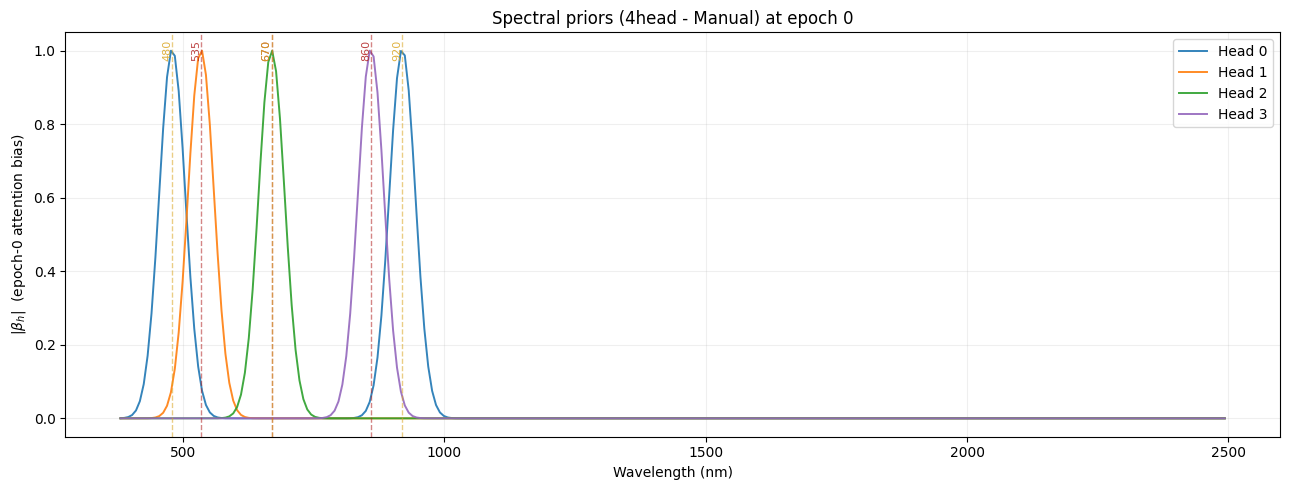
\includegraphics[width=\linewidth]{4head_manualprior.png}\\[0.5em]
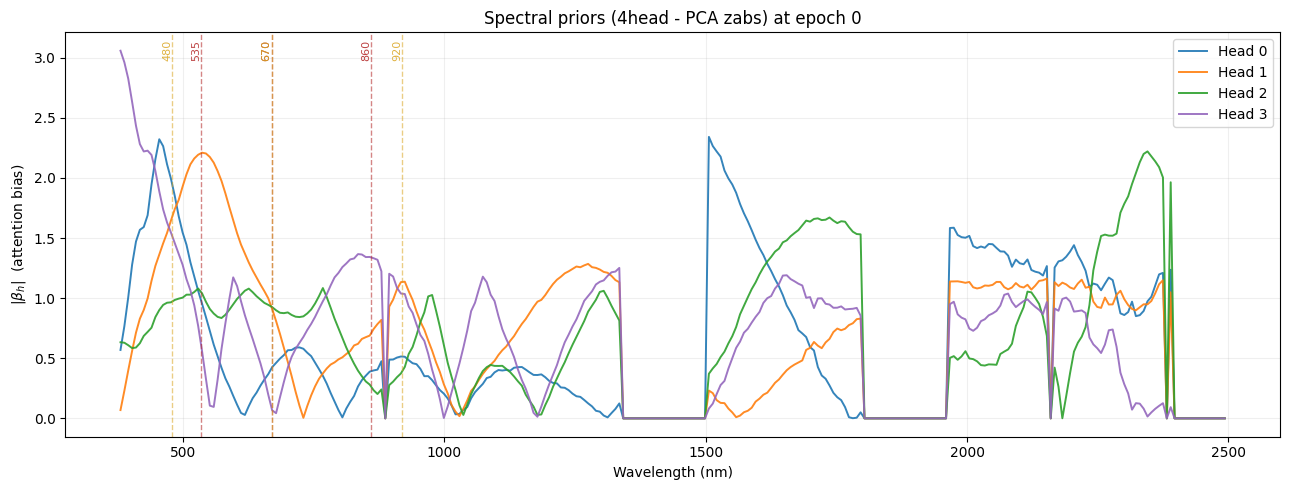
\includegraphics[width=\linewidth]{4head_PCAzabprior.png}
\caption{Attention bias $|\bm{\beta}_h|$ at epoch 0 (initialization) for the two architectural-prior constructions at $H = 4$. \textbf{Top:} manual diagnostic-band prior, with Gaussian bumps centered at literature Fe$^{3+}$ wavelengths (480, 535, 670, 860, 920~nm) assigned round-robin to heads. \textbf{Bottom:} PCA-curated prior (\texttt{zabs} normalization) derived from the four leading principal components of the curated iron-bearing reference library; non-zero across most unmasked bands, with sharp drop-outs at the water-vapor mask edges. Vertical dashed lines mark the same five literature wavelengths in both panels for visual reference. The two priors differ by $\sim$50$\times$ in spectral support and $\sim$3$\times$ in peak magnitude, yet both reach the same final top-1 accuracy at $H = 4$ (Section~\ref{sec:ablation}).}
\label{fig:prior_init_compare}
\end{figure}

\subsubsection{Water vapor band masking}
\label{sec:wv_mask}

Atmospheric water vapor absorption at $\sim$1340--1500~nm and $\sim$1800--1960~nm dominates TOA reflectance variance but carries no mineralogical information for Group~1 iron-oxide targets, whose diagnostic features all lie at 480--920~nm. A boolean mask $\mathbf{m} \in \{0, 1\}^L$ zeroes the prior at atmospheric bands during construction and pins $\bm{\beta}_{h,j}$ at zero in those bands during the trainable post-freeze phase via $\bm{\beta}_{h,j} \leftarrow \bm{\beta}_{h,j} m_j$ on every optimizer step. The mask thus serves a specific role for prior-bearing configurations: it prevents the trainable bias from drifting into H$_2$O bands and absorbing atmospheric noise as a free degree of freedom. Empirically, removing the mask from a prior-bearing 4-head run causes $\|\bm{\beta}\|_{\text{rms}}$ to amplify by $\sim$54\% (driven by H$_2$O-band drift) and top-1 accuracy to drop $\sim$1.6~pp. For configurations without a trainable bias (transformer-only baseline) or with their own consistency-loss regularization (LUSI, Section~\ref{sec:lusi}), the mask plays no equivalent role and is dropped.

\subsubsection{Hybrid head allocation and freeze schedule}
\label{sec:hybrid_heads}

When $H > k$ PCA components, the first $k$ heads are prior-initialized and the remaining $H - k$ are zero-initialized. Per Equation~\ref{eq:attn_score}, zero-initialized heads begin with uniform attention; symmetry across them is broken by the random query vectors $\mathbf{q}_h \sim \mathcal{N}(\mathbf{0}, \mathbf{I})$, so explicit noise on the bias is unnecessary. Prior-bearing heads are frozen for a user-specified initial number of epochs (default 3), allowing the classification head to establish a baseline mapping from the physics-derived features before fine-tuning; zero-initialized heads (and the manual-prior heads) train from epoch~1.

%% ====================================================================
%% 6.X LUSI CONSISTENCY REGULARIZATION (subsection of Optional extensions)
%% ====================================================================
\subsection{Learning Using Statistical Invariants (LUSI)-inspired consistency reglarization}
\label{sec:lusi}

LUSI \cite{vapnik2020} encourages predictions to remain stable under physical transformations that should not change mineral identity.
LUSI injects domain knowledge through the loss function and can be used independently or in combination with PCA spectral priors.

\subsubsection{Theoretical background}

Section~\ref{subsec:physics_informed_approaches} positions LUSI in the broader physics-informed-learning literature. To recap briefly: in Vapnik and Izmailov's original formulation~\cite{vapnik2020}, domain knowledge enters as \emph{predicates} and \emph{statistical invariants} that restrict the admissible function class --- hard constraints on what the learned function must satisfy. The neural training setting does not directly admit such hard constraints, so this work implements a transformation-based approximation: physically motivated transformations are applied to the input spectrum, and the model is penalized for changes in its prediction under those transformations. The penalty is realized as a teacher--student consistency objective borrowed from knowledge distillation~\cite{hinton2015distilling}: the model's prediction on the original (untransformed) spectrum acts as a fixed \emph{teacher} target with gradients stopped, while the prediction on the transformed spectrum is the \emph{student}, trained to match the teacher.

The physical motivation for the transformations comes from the fact that TOA reflectance is a transformed version of surface reflectance, not an equivalent quantity. Under the first-order TOA decomposition (Equation~\ref{eq:toa_decomp}), changes in illumination, atmospheric transmittance ($T_{\downarrow} T_{\uparrow}$), and path reflectance ($\rho_{\mathrm{path}}$) can alter the observed TOA spectrum without changing the underlying mineral identity. The LUSI transformations approximate these effects directly in the TOA-observation domain: the scale transformation $T_{\text{scale}}$ (Equation~\ref{eq:scale_predicate}) represents broadband multiplicative changes in brightness, while the slope-change transformation $T_{\text{slope}}$ (Equation~\ref{eq:slope_predicate}) represents a conservative low-frequency additive spectral-slope perturbation. These transformations are therefore not an atmospheric-correction model and do not assume $\rho_{\mathrm{toa}} \approx \rho_{\mathrm{surface}}$; rather, they define label-preserving directions in TOA reflectance space along which the predicted mineral label should remain stable.

\subsubsection{Physical predicates}
\label{sec:lusi_predicates}

The two transformations approximate label-preserving modes of variation suggested by the TOA decomposition in Equation~\ref{eq:toa_decomp}:

\paragraph{Illumination invariance}
Topographic slope and partial shadow scale TOA reflectance by a multiplicative factor without altering the diagnostic spectral shape. (Solar zenith angle is already accounted for in the TOA reflectance conversion via the $\cos\theta$ normalization in Section~\ref{sec:radiance_toa}, but a tilted surface receives more or less direct illumination than this flat-surface correction assumes.)
\begin{equation}
T_{\text{scale}}(\mathbf{w}) = \rho \mathbf{w}, \quad \rho \sim \mathcal{U}(0.8, 1.2).
\label{eq:scale_predicate}
\end{equation}
A uniform distribution is chosen because there is no reason to favor any particular illumination level within the range; $\pm$20\% spans the typical brightness variation from topographic slope and shadow effects observed in EMIT scenes over arid terrain. In EMIT's study regions (Sahara, Arabian Peninsula, Horn of Africa), mountain ranges and dune fields produce significant relief, making slope-induced brightness variation a common occurrence.

\paragraph{Atmospheric slope invariance}
Aerosol and Rayleigh effects can introduce low-frequency spectral-shape changes that are not diagnostic of mineral identity.
After robust normalization, these effects are approximated by a small additive wavelength ramp:
\begin{equation}
T_{\text{slope}}(\mathbf{w}) = \mathbf{w} + \xi \boldsymbol{\lambda}_{\text{grid}}, \quad \xi \sim \mathcal{N}(0, 0.01),
\label{eq:slope_predicate}
\end{equation}
where $\boldsymbol{\lambda}_{\text{grid}} = \mathrm{linspace}(-1, 1, L)$.
This is not intended to be a full atmospheric model; it is a conservative label-preserving perturbation that encourages invariance to smooth spectral-slope changes while preserving narrow mineral absorption structure.

\paragraph{Joint transformation.}
The two predicates are applied jointly:
\begin{equation}
T_{\text{joint}}(\mathbf{w}) = \rho \mathbf{w} + \xi \boldsymbol{\lambda}_{\text{grid}},
\label{eq:joint_transform}
\end{equation}
with $\rho$ and $\xi$ sampled independently per sample.

\subsubsection{Consistency loss}
\label{sec:lusi_loss}

The LUSI loss measures whether the model's mineral classification changes when the input spectrum is physically transformed. The model is run twice on each training batch:
\begin{enumerate}
  \item \textbf{Original spectrum} $\mathbf{w}$ (``teacher''): the untransformed input, producing prediction $\mathbf{p}_{\text{orig}} = \text{Softmax}(\text{logits}_{\text{orig}} / \tau_l) \in \R^{Q_1}$.
  \item \textbf{Transformed spectrum} $T_{\text{joint}}(\mathbf{w})$ (``student''): the same pixel after applying the scale and slope-change perturbations (Equation~\ref{eq:joint_transform}), producing prediction $\mathbf{p}_{\text{trans}} = \text{Softmax}(\text{logits}_{\text{trans}} / \tau_l) \in \R^{Q_1}$.
\end{enumerate}
The consistency loss compares the softened prediction for the transformed spectrum to the stop-gradient prediction for the original spectrum:
\begin{equation}
\mathcal{L}_{\text{LUSI}} =
D_{\text{KL}}\!\left(
\mathbf{p}_{\text{orig}}^{\mathrm{sg}}
\,\|\,
\mathbf{p}_{\text{trans}}
\right)\,\tau_l^{2},
\label{eq:lusi_kl}
\end{equation}
where $\mathbf{p}_{\text{orig}}^{\mathrm{sg}}$ denotes the original prediction with gradients stopped, $\tau_l = 2.0$ is a softening temperature, and the $\tau_l^{2}$ factor follows the knowledge-distillation convention \cite{hinton2015distilling}, compensating for the smaller KL magnitude that softer distributions produce so the gradient scale stays comparable to the cross-entropy term. The stop-gradient anchors the teacher to the model's current prediction on the clean input; this trains the transformed-input prediction to match the original-input prediction without allowing the loss to be minimized by drifting both predictions toward a shared trivial answer. The total loss is:
\begin{equation}
\mathcal{L}_{\text{total}} = \mathcal{L}_{\text{CE}} + \lambda_{\text{LUSI}} \mathcal{L}_{\text{LUSI}},
\label{eq:lusi_total}
\end{equation}
with $\lambda_{\text{LUSI}} = 1.0$.

In practice, LUSI is applied as a data-augmentation step at every training iteration. For each batch of $B$ pixels, the implementation samples a fresh pair $(\rho_i, \xi_i)$ \emph{independently for every pixel} --- $\rho_i \sim \mathcal{U}(0.8, 1.2)$ and $\xi_i \sim \mathcal{N}(0, 0.01)$ --- and applies the joint transformation $T_{\text{joint}}(\mathbf{w}_i) = \rho_i \mathbf{w}_i + \xi_i \boldsymbol{\lambda}_{\text{grid}}$. Because the data loader shuffles between epochs, each physical pixel is sampled into a different batch each pass, and a different $(\rho_i, \xi_i)$ is drawn each time it appears. Across the full 120-epoch training run, the same pixel is therefore seen by the model under $\sim$120 different random perturbations, and the consistency loss pushes the model to produce the same class prediction for all of them. The same pixel always carries the same true mineral label for the cross-entropy loss; only the LUSI augmentation varies. This is the same per-iteration data-augmentation pattern used in image classification (random crops, flips, colour jitter), specialized to the spectral domain.

LUSI requires two additional forward passes per batch, approximately doubling training time.

\subsubsection{Empirical findings}
\label{sec:lusi_findings}

LUSI does not improve accuracy on the training distribution: 4-head LUSI-only (0.773) underperforms the transformer baseline (0.791), and 8-head PCA+LUSI (0.805) matches PCA-only (0.806) within noise.
The LUSI loss converges to $\sim$0.03, indicating the model already achieves brightness/slope invariance through standard training at the $\sim$1M pixel data scale.

Cross-region deployment to a geographically disjoint southwestern US desert region (20 mineral-populated granules) reduces top-1 accuracy by $8$--$17$~pp from the training-region validation pool, while top-3 accuracy stays in the $0.87$--$0.92$ range across all configurations (Table~\ref{tab:crossscene}). At $H = 4$ the manual prior leads cross-region (SW top-1 $= 0.724$, $-8.4$~pp drop), $+5.5$~pp above the unguided baseline and $+9.0$~pp above LUSI. At $H = 8$ the PCA-curated prior leads (SW top-1 $= 0.705$, $-11.3$~pp drop), narrowly above Manual 8H ($0.699$) and well above LUSI 8H ($0.666$). The 4H winner is the sharp manual prior; the 8H winner is the diffuse PCA-curated prior --- the sharp-vs-diffuse split at different head counts mirrors the in-distribution pattern of Table~\ref{tab:ablation}. Architectural priors are the consistent cross-region winners; LUSI is last or next-to-last on both top-1 and top-3 at both head counts in this evaluation.

\begin{table}[!htbp]
\centering
\small
\caption{Cross-region deployment. Train columns report the held-out validation-pool accuracy from Table~\ref{tab:ablation} on Africa/Middle East pixels. SW columns report the mean accuracy across 20 SW US granules each containing at least $20\%$ Group-1 mineral pixels, under full-granule inference. Bold marks the leader within each head-count block on each SW metric.}
\label{tab:crossscene}
\begin{tabular}{p{0.24\linewidth}p{0.13\linewidth}p{0.13\linewidth}p{0.13\linewidth}p{0.13\linewidth}}
\hline
\rowcolor[gray]{0.85}
\textbf{Configuration} & \textbf{Train top-1} & \textbf{SW top-1} & \textbf{Train top-3} & \textbf{SW top-3} \\
\hline
Trans 4H & 0.789 & 0.669 & 0.961 & 0.877 \\
\hline
\textbf{Manual 4H} & 0.808 & \textbf{0.724} & 0.967 & \textbf{0.919} \\
\hline
PCA-zabs 4H & 0.809 & 0.644 & 0.967 & 0.868 \\
\hline
LUSI 4H & 0.787 & 0.634 & 0.961 & 0.875 \\
\hline
Trans 8H & 0.819 & 0.683 & 0.970 & 0.902 \\
\hline
Manual 8H & 0.806 & 0.699 & 0.966 & 0.896 \\
\hline
\textbf{PCA-zabs 8H} & 0.818 & \textbf{0.705} & 0.970 & \textbf{0.910} \\
\hline
LUSI 8H & 0.796 & 0.666 & 0.962 & 0.893 \\
\hline
\end{tabular}
\end{table}

%% ====================================================================
%% 8. ABLATION
%% ====================================================================
\section{Ablation: manual spectral prior vs.\ transformer-only baseline}
\label{sec:ablation}

This section evaluates the manual spectral prior of Section~\ref{sec:manual_priors} against the transformer-only baseline of Section~\ref{sec:trans_only_results} at two head counts ($H = 4$ and $H = 8$).
All four configurations were trained for 120 epochs on the same 1.26~million pixel training set with identical optimizer settings, the same fixed random seed, and the same hardware (Apple M4 Max, MPS backend); the only differences are the number of attention heads and whether the attention bias $\bm{\beta}_h$ was initialized to zero (transformer-only) or to the round-robin Gaussian-bump pattern at the canonical Fe$^{3+}$ wavelengths from Table~\ref{tab:fe_diagnostics} (manual prior, $\alpha = 1.0$, freeze=3 epochs).

\paragraph{Headline finding.}
A 4-head transformer initialized with the manual spectral prior (top-1 = 0.808, train+val 117 min) delivers $1.9$ of the $3.0$~percentage-point gain that doubling the head count produces (Trans $H = 4$: $0.789 \to$ Trans $H = 8$: $0.819$, 134 min) --- approximately $63\%$ of the head-doubling benefit at zero additional training time, and a useful operating point when training compute is constrained. Crucially, the transformer baseline at $H = 4$ uses a trainable attention bias initialized at zero, parameter-matched to the prior-bearing configurations, so the prior's $+1.9$~pp gain over this baseline is unambiguously attributable to the spectroscopic initialization rather than to added trainable parameters or differential preprocessing. Table~\ref{tab:ablation} reports the full ablation, including PCA-curated and LUSI variants at $H = 4$ and $H = 8$.

\begin{table}[!htbp]
\centering
\small
\caption{Ablation of the two physics-injection mechanisms at $H=4$ and $H=8$.
All runs use the same data split, optimizer settings, derivative tokenization, learned query vectors, and trainable per-head attention bias $\bm{\beta}_h$.
The transformer baseline initializes $\bm{\beta}_h$ at zero.
Manual and PCA-curated configurations initialize $\bm{\beta}_h$ from Fe$^{3+}$ diagnostic wavelengths or curated USGS-library PCA loadings, respectively.
LUSI uses zero-initialized trainable bias and adds only the statistical-invariance consistency loss.
Wall-clock timings are for full training and validation on a single Apple M4 Max laptop using PyTorch MPS.}
\label{tab:ablation}
\begin{tabular}{p{0.30\linewidth}p{0.08\linewidth}p{0.13\linewidth}p{0.13\linewidth}p{0.18\linewidth}}
\hline
\rowcolor[gray]{0.85}
\textbf{Configuration} & \textbf{\#Heads} & \textbf{Top-1 Acc.} & \textbf{Top-3 Acc.} & \textbf{Train + Val Time (min)} \\
\hline
Transformer baseline & 4 & 0.789 & 0.961 & 119 \\
\hline
\textbf{Manual prior (Fe$^{3+}$ bands)} & \textbf{4} & \textbf{0.808} & \textbf{0.967} & \textbf{117} \\
\hline
PCA-curated prior & 4 & 0.809 & 0.967 & 124 \\
\hline
LUSI-only & 4 & 0.787 & 0.961 & 289 \\
\hline
PCA-curated + LUSI & 4 & 0.790 & 0.962 & $\sim$290 \\
\hline
Transformer baseline & 8 & 0.819 & 0.970 & 134 \\
\hline
Manual prior (Fe$^{3+}$ bands) & 8 & 0.806 & 0.966 & 125 \\
\hline
PCA-curated prior & 8 & 0.818 & 0.970 & 129 \\
\hline
LUSI-only & 8 & 0.796 & 0.962 & 326 \\
\hline
\end{tabular}
\end{table}
At $H = 8$ the manual prior \emph{underperforms} the parameter-matched transformer baseline by $-1.3$~pp ($0.819 \to 0.806$). This is the cleanest possible realization of the standard observation that physics-informed priors help most when the model's capacity is constrained \cite{raissi2019pinn, karpatne2017tgds}: in the capacity-constrained regime ($H = 4$) the prior is a substantial inductive scaffold, while in the capacity-saturated regime ($H = 8$) the same scaffold becomes a mild over-constraint. The unguided 8-head model already discovers most of the diagnostic regions on its own --- the red trace in Figure~\ref{fig:trans4_attn} hits the visible Fe$^{3+}$ region in Head~1 and the NIR continuum near canonical 860~nm in Head~3 at $H = 4$, and the corresponding $H = 8$ baseline picks up additional regions through its extra heads.

\paragraph{Why the 8-head manual prior underperforms 8-head transformer-only.}
Two structural observations from training diagnostics support the capacity-saturation interpretation.
First, the attention-bias RMS magnitude $\|\bm{\beta}\|_{\text{rms}}$ at the end of training was $0.977$ for the $H = 4$ manual run --- essentially unchanged from its initialization at $\alpha = 1.0$ --- but rose to $1.154$ for the $H = 8$ manual run, indicating that the eight-head model amplified the prior-anchored heads during training rather than discovering complementary features through the three additional random heads.
Second, the average pairwise cosine similarity between heads' learned query vectors $\mathbf{q}_h$ was $0.015$ for $H = 8$ versus $0.031$ for $H = 4$, ruling out head collapse as an explanation: the random heads stayed distinct from the prior-anchored heads but the model elected not to use that capacity for novel feature discovery.

\paragraph{Sharp vs. diffuse architectural priors at saturated capacity.}
The PCA-curated prior at $H = 8$ reaches top-1 $0.818$, statistically tied with the parameter-matched transformer baseline ($0.819$) rather than underperforming it: its diffuse non-zero loadings span $\sim$220 of 285 bands and align with the variance directions the unguided model would discover anyway, leaving the prior neutral rather than constraining at $H = 8$. Diagnostically, $\|\bm{\beta}\|_{\text{rms}} = 1.066$ for the $H = 8$ PCA-curated run, barely above its $\alpha = 1.0$ initialization, versus $1.154$ for the manual run --- the manual prior amplifies more aggressively because the model has to lean into its narrow bumps to use them, while PCA-curated barely amplifies above its initial scale. The capacity-saturation harm is therefore sharpness-dependent: \emph{sharp} architectural priors (Manual, 5 narrow Gaussian bumps) become mildly over-constraining at saturated capacity, while \emph{diffuse} architectural priors (PCA-curated, broad band coverage) become neutral. Together these observations sharpen the headline takeaway: \emph{architectural priors are most valuable as a way to compress capacity, and at saturated capacity their cost depends on how concentrated their spectral support is}.

\paragraph{Combining architectural and loss-based priors causes interference at constrained capacity.}
A combined PCA-curated~+~LUSI run at $H = 4$ reaches top-1 $0.790$ --- $1.9$~percentage points \emph{below} PCA-curated alone ($0.809$) and statistically tied with the unguided baseline. The interference is mechanically visible in the bias diagnostics: the trainable bias amplified to $\|\bm{\beta}\|_{\text{rms}} = 1.648$, well above either prior construction alone (PCA-curated: $0.946$; LUSI alone: $1.308$). LUSI's consistency loss appears to use the bias as a buffer between augmented and un-augmented passes, distorting the structured PCA initialization. The two priors target different failure modes --- architectural priors for in-distribution accuracy by structured initialization, loss-based priors for cross-region robustness by predicate invariance --- and at constrained capacity ($H = 4$) the two pressures conflict rather than stack additively. The corresponding $H = 8$ combined configuration was not re-evaluated under the current parameter-matched pipeline; the legacy 8-head PCA+LUSI run reported in earlier project notes reached $0.805$, statistically tied with the legacy 8-head PCA-only run at $0.806$, which is consistent with the conjecture that the interference is capacity-dependent.

\paragraph{Convergence trajectories across all configurations.}
Figure~\ref{fig:earlyepoch} compares the full 120-epoch training trajectories across all nine configurations of the ablation. Three tiers emerge visually: an upper 8H tier comprising the transformer baseline and the PCA-curated prior ($\sim$0.818--0.819, tracking each other closely throughout); a mid tier of 4H architectural-prior runs and 8H Manual ($\sim$0.806--0.809); and a 4H bottom cluster comprising the unguided baselines, the LUSI-only run, and the interfering PCA+LUSI combination ($\sim$0.787--0.790). The 8H LUSI configuration sits alone at $\sim$0.796 between the mid tier and the 4H bottom cluster, reflecting the in-distribution penalty of loss-based regularization at saturated capacity.

\begin{figure}[!htbp]
\centering
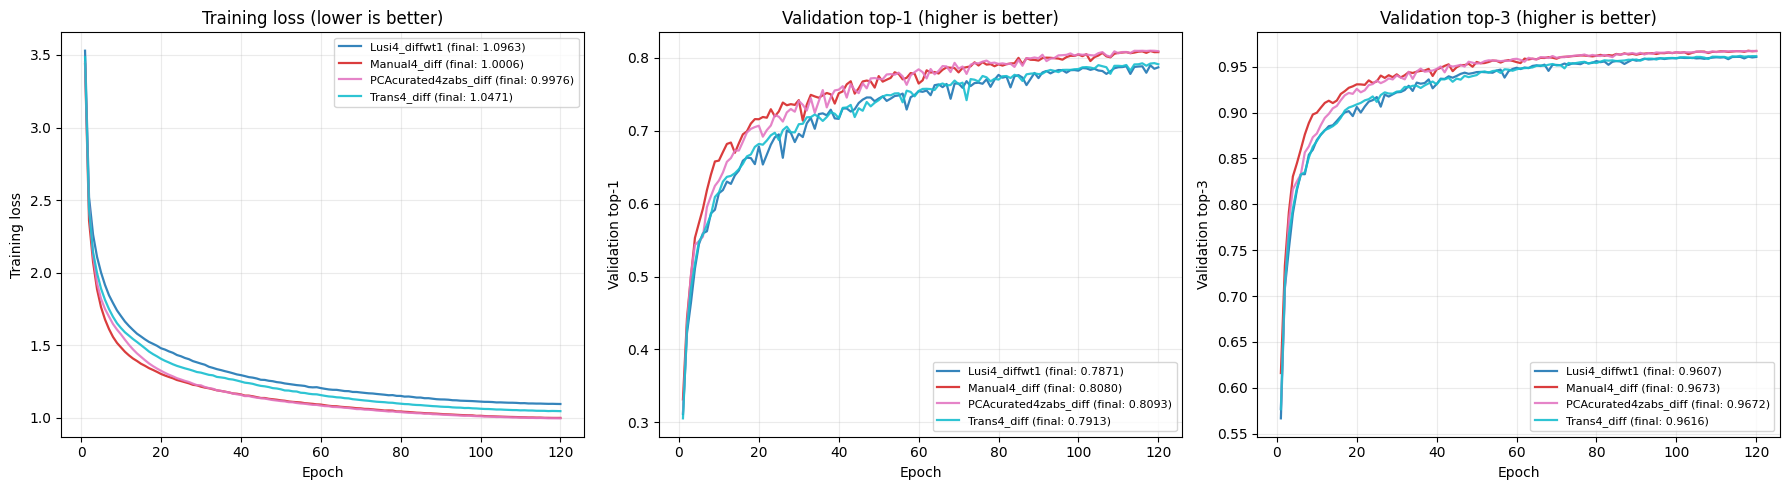
\includegraphics[width=\textwidth]{train_top1_top3.png}
\caption{Convergence trajectories for the nine configurations of the ablation. \textbf{Left:} training cross-entropy loss (lower is better). \textbf{Center:} validation top-1. \textbf{Right:} validation top-3. Legend reports the final-epoch value. Three tiers are visually distinct: 8H transformer baseline and 8H PCA-curated \texttt{zabs} prior at the top ($\sim$0.818--0.819); 4H architectural-prior runs and 8H Manual mid-table ($\sim$0.806--0.809); 4H baselines and the 4H PCA+LUSI combination forming the bottom cluster ($\sim$0.787--0.790), with 8H LUSI alone in between ($\sim$0.796).}
\label{fig:earlyepoch}
\end{figure}

\paragraph{Caveats.}
The reported numbers are single-seed runs at one training-set size ($N \approx 1.26 \times 10^{6}$).
At smaller training sizes the prior would be expected to provide larger gains (consistent with prior-as-capacity-substitute interpretation), and at larger training sizes the gap should shrink further --- a direct test of this would require re-running the full ablation at $N = 10^4, 10^5, 10^6$ pixels, which is left for future work.
These manual-prior runs do not include LUSI (Section~\ref{sec:lusi}); LUSI's combined effect with the manual prior is reported separately in Section~\ref{sec:lusi_findings}.

\paragraph{Rarity analysis: where the prior's accuracy gain comes from.}
The headline accuracy comparison treats every Group~1 class equally, but the per-class training-set support spans nearly four orders of magnitude (1 to 7{,}500 pixels per class after the stratified cap). Figure~\ref{fig:rarity_grid} stratifies per-class precision, recall, and F1 by training-set support across three rarity bins, with one bar per configuration. The picture is striking: at the rare end (150--1000 training samples), Manual~4H reaches F1 = 0.62, statistically tied with the 8-head transformer baseline (F1 = 0.64) and substantially above LUSI~4H (F1 = 0.49) --- a $+13$~pp F1 advantage of the architectural prior over the loss-based prior in the rare-class regime. At the common end (1000--4000 training samples), all eight configurations cluster at F1 = 0.82--0.86 with negligible separation. The architectural prior's accuracy gain is therefore concentrated in the rare-class regime, exactly where the canonical PINN-tradition prediction expects physics-informed initialization to help most. Practically, this localizes the headline ``Manual 4H matches Trans 8H'' result: it is a rare-class equivalence, not a uniform gain across class frequencies, and Manual~4H buys the head-doubling benefit specifically on rare-class generalization at no extra training cost.

\begin{figure}[!htbp]
\centering
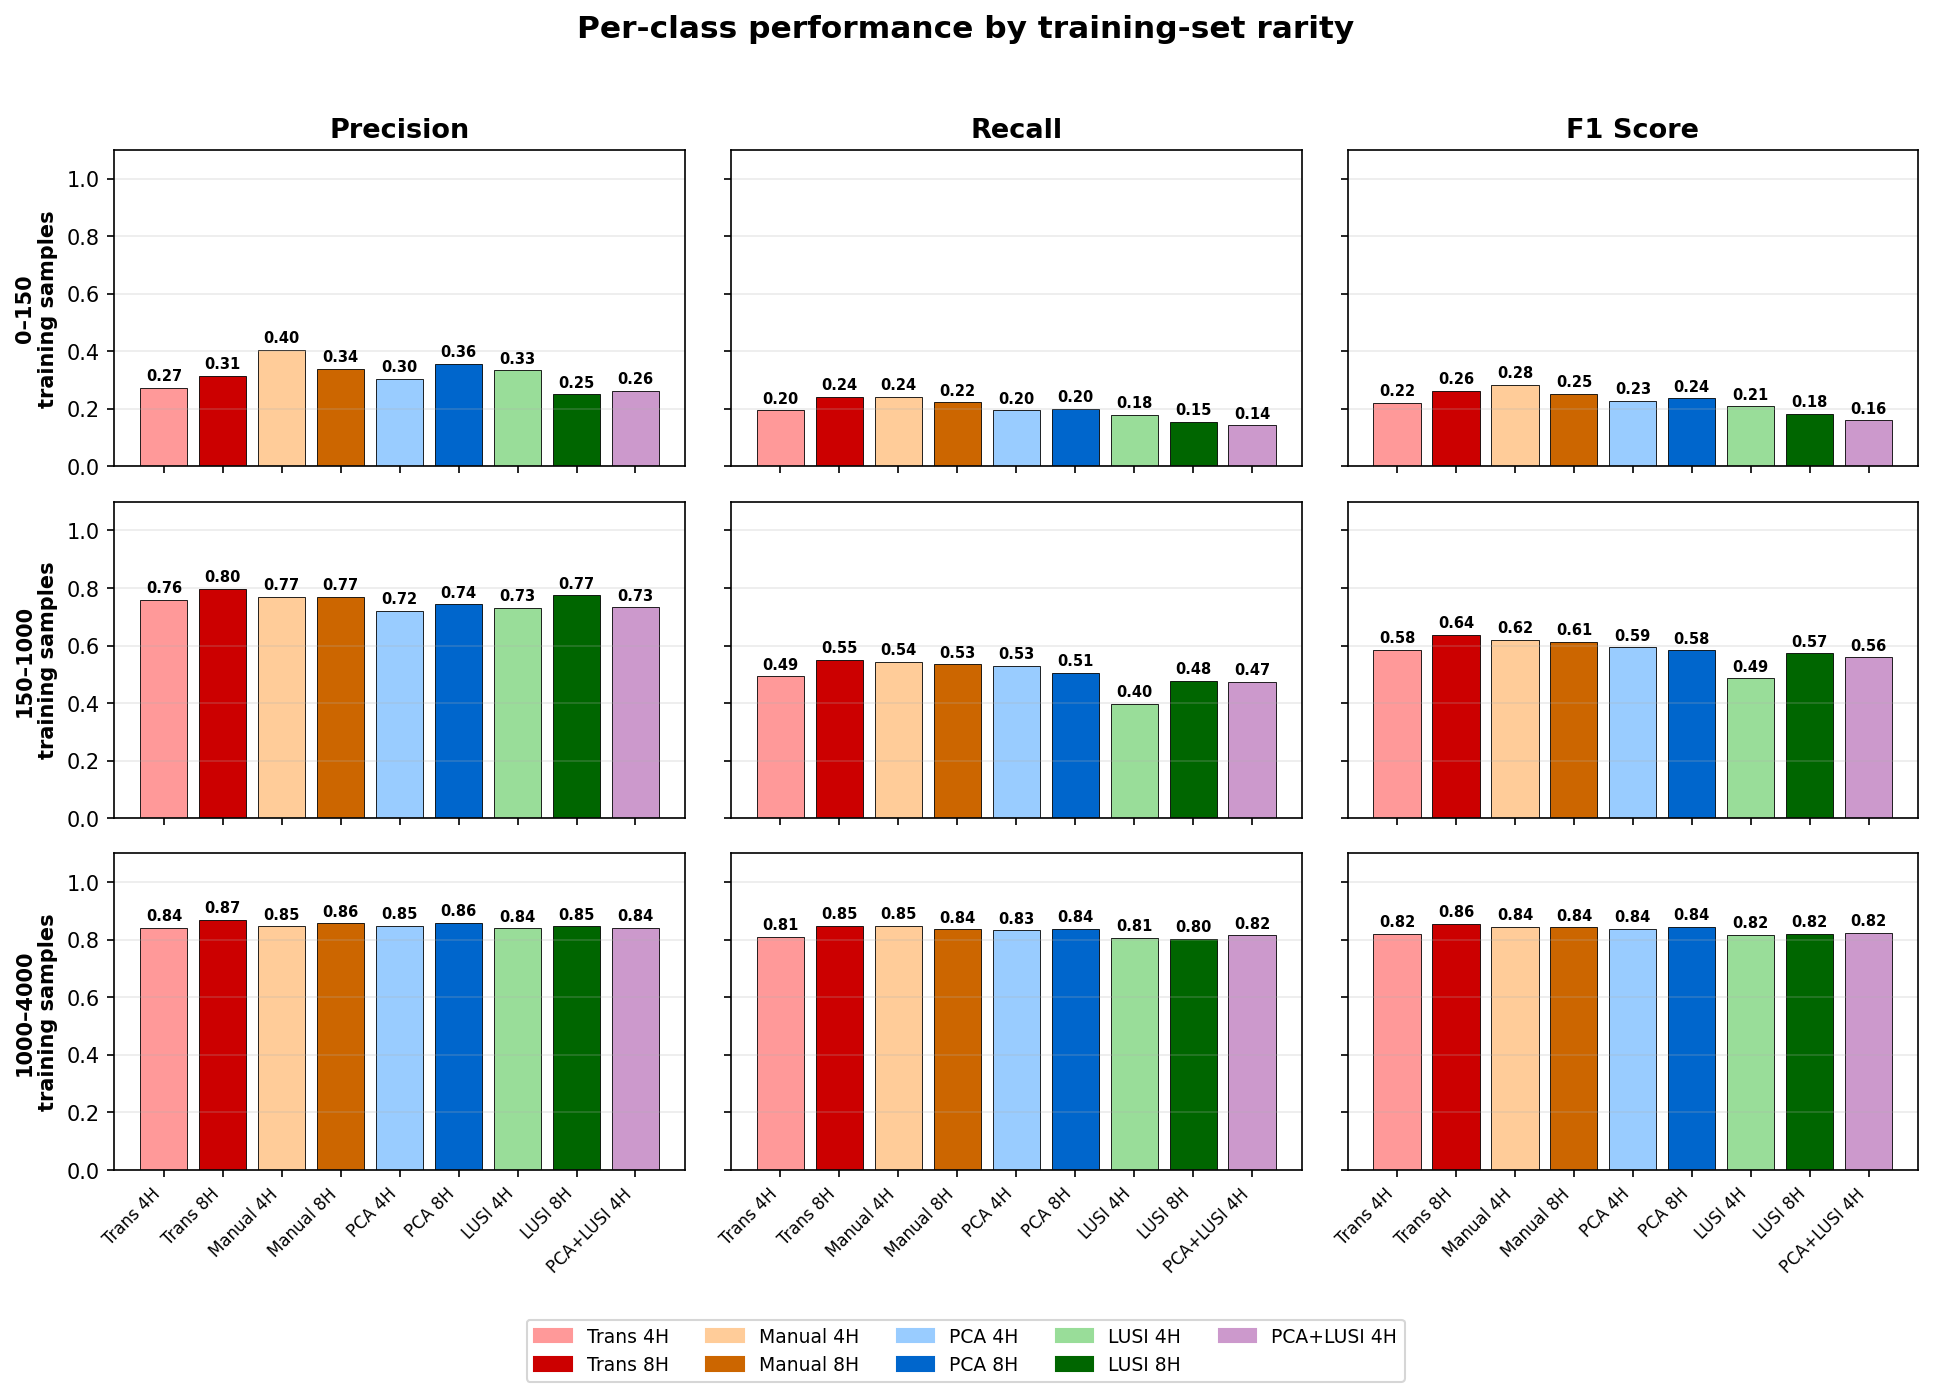
\includegraphics[width=\textwidth]{comparison_rarity_grid.png}
\caption{Per-class precision, recall, and F1-score stratified by training-set support across three rarity bins, for the eight 4H and 8H configurations of Table~\ref{tab:ablation} (the PCA+LUSI 4H combined run is omitted for visual clarity). \textbf{Rows:} rarity bins (0--150, 150--1000, 1000--4000 training pixels per class). \textbf{Columns:} precision, recall, F1. The architectural-prior advantage is concentrated in the rare-class regime: Manual~4H reaches F1 = 0.62 in the 150--1000 bin, tied with the 8-head transformer baseline at F1 = 0.64 and well above LUSI~4H at F1 = 0.49. At the common end (1000--4000 samples) all configurations converge to F1 = 0.82--0.86, suggesting the prior's contribution is largely exhausted once classes have enough training data for the unguided model to discover the structure on its own. Bin edges and axis ranges chosen to highlight the regime where configurations diverge.}
\label{fig:rarity_grid}
\end{figure}

\section{Full-image granule inference}
\label{sec:full_image_inference}

The held-out validation pool of Section~\ref{sec:trans_only_results} draws random pixels from across all 396 training granules and inherits the class-balanced training distribution (7,500-pixel cap per ID). At deployment, however, the model is applied to a single EMIT granule whose mineralogy is not class-balanced --- two or three classes typically account for $80$--$99\%$ of mineral pixels --- and the relevant question is whether the validation accuracy of Table~\ref{tab:ablation} transfers to that setting. Four granules were evaluated under all four locked $H = 4$ configurations: Image~0 (163{,}391 mineral pixels, atypical class-28 distribution); Image~4 (1{,}589{,}704 mineral pixels, classes 47/45/28 = $99\%$); Image~50 (1{,}445{,}153 mineral pixels, goethite-dominated 8/46/40 = $87\%$); Image~100 (1{,}589{,}760 mineral pixels, goethite-dominated 8/46/7/45/49 = $99\%$). Inference takes $\sim$45~seconds per granule on the same hardware as training.

Across the three deployment-realistic granules (Images~4, 50, 100), the mean top-1 ranking is PCA-curated (0.888) $>$ Manual (0.882) $>$ Trans (0.874) $>$ LUSI (0.865) --- the same ordering as the validation pool, with the same magnitude of separation between architectural priors and the unguided baseline ($\sim$1--2~pp). Macro recall favors the architectural priors on every granule (the unguided transformer never has the highest macro recall), and rare-class lift is visible at granule scale: on Image~50, classes 21 and 22 ($\sim$1{,}500 pixels each) gain $+22$--$24$~pp F1 under the architectural prior; on Image~100, class~32 (117 pixels) jumps from F1 = $0.04$ (Trans) to $0.32$ (PCA-curated). Top-3 saturates on representative granules ($0.987$--$0.999$ across all configs); top-1 and macro F1 are the discriminating metrics at deployment scale. Image~0 is a deployment-failure case for the architectural priors --- PCA-curated scores F1 = $0.49$ on class~28 in this granule versus $0.95$ on Image~4 with the same checkpoint, because the granule's class-28 pixels deviate from the canonical Fe-hydroxide spectroscopic signature and the prior-bearing models pull back rather than commit. This is the granule-scale analog of the cross-region degradation pattern: priors crisp up canonical pixels and trade some accuracy on atypical ones. LUSI~4H is the lowest top-1 on every granule and on the validation pool; its distinguishing advantage remains cross-region robustness rather than in-distribution accuracy.

\begin{figure}[!htbp]
\centering
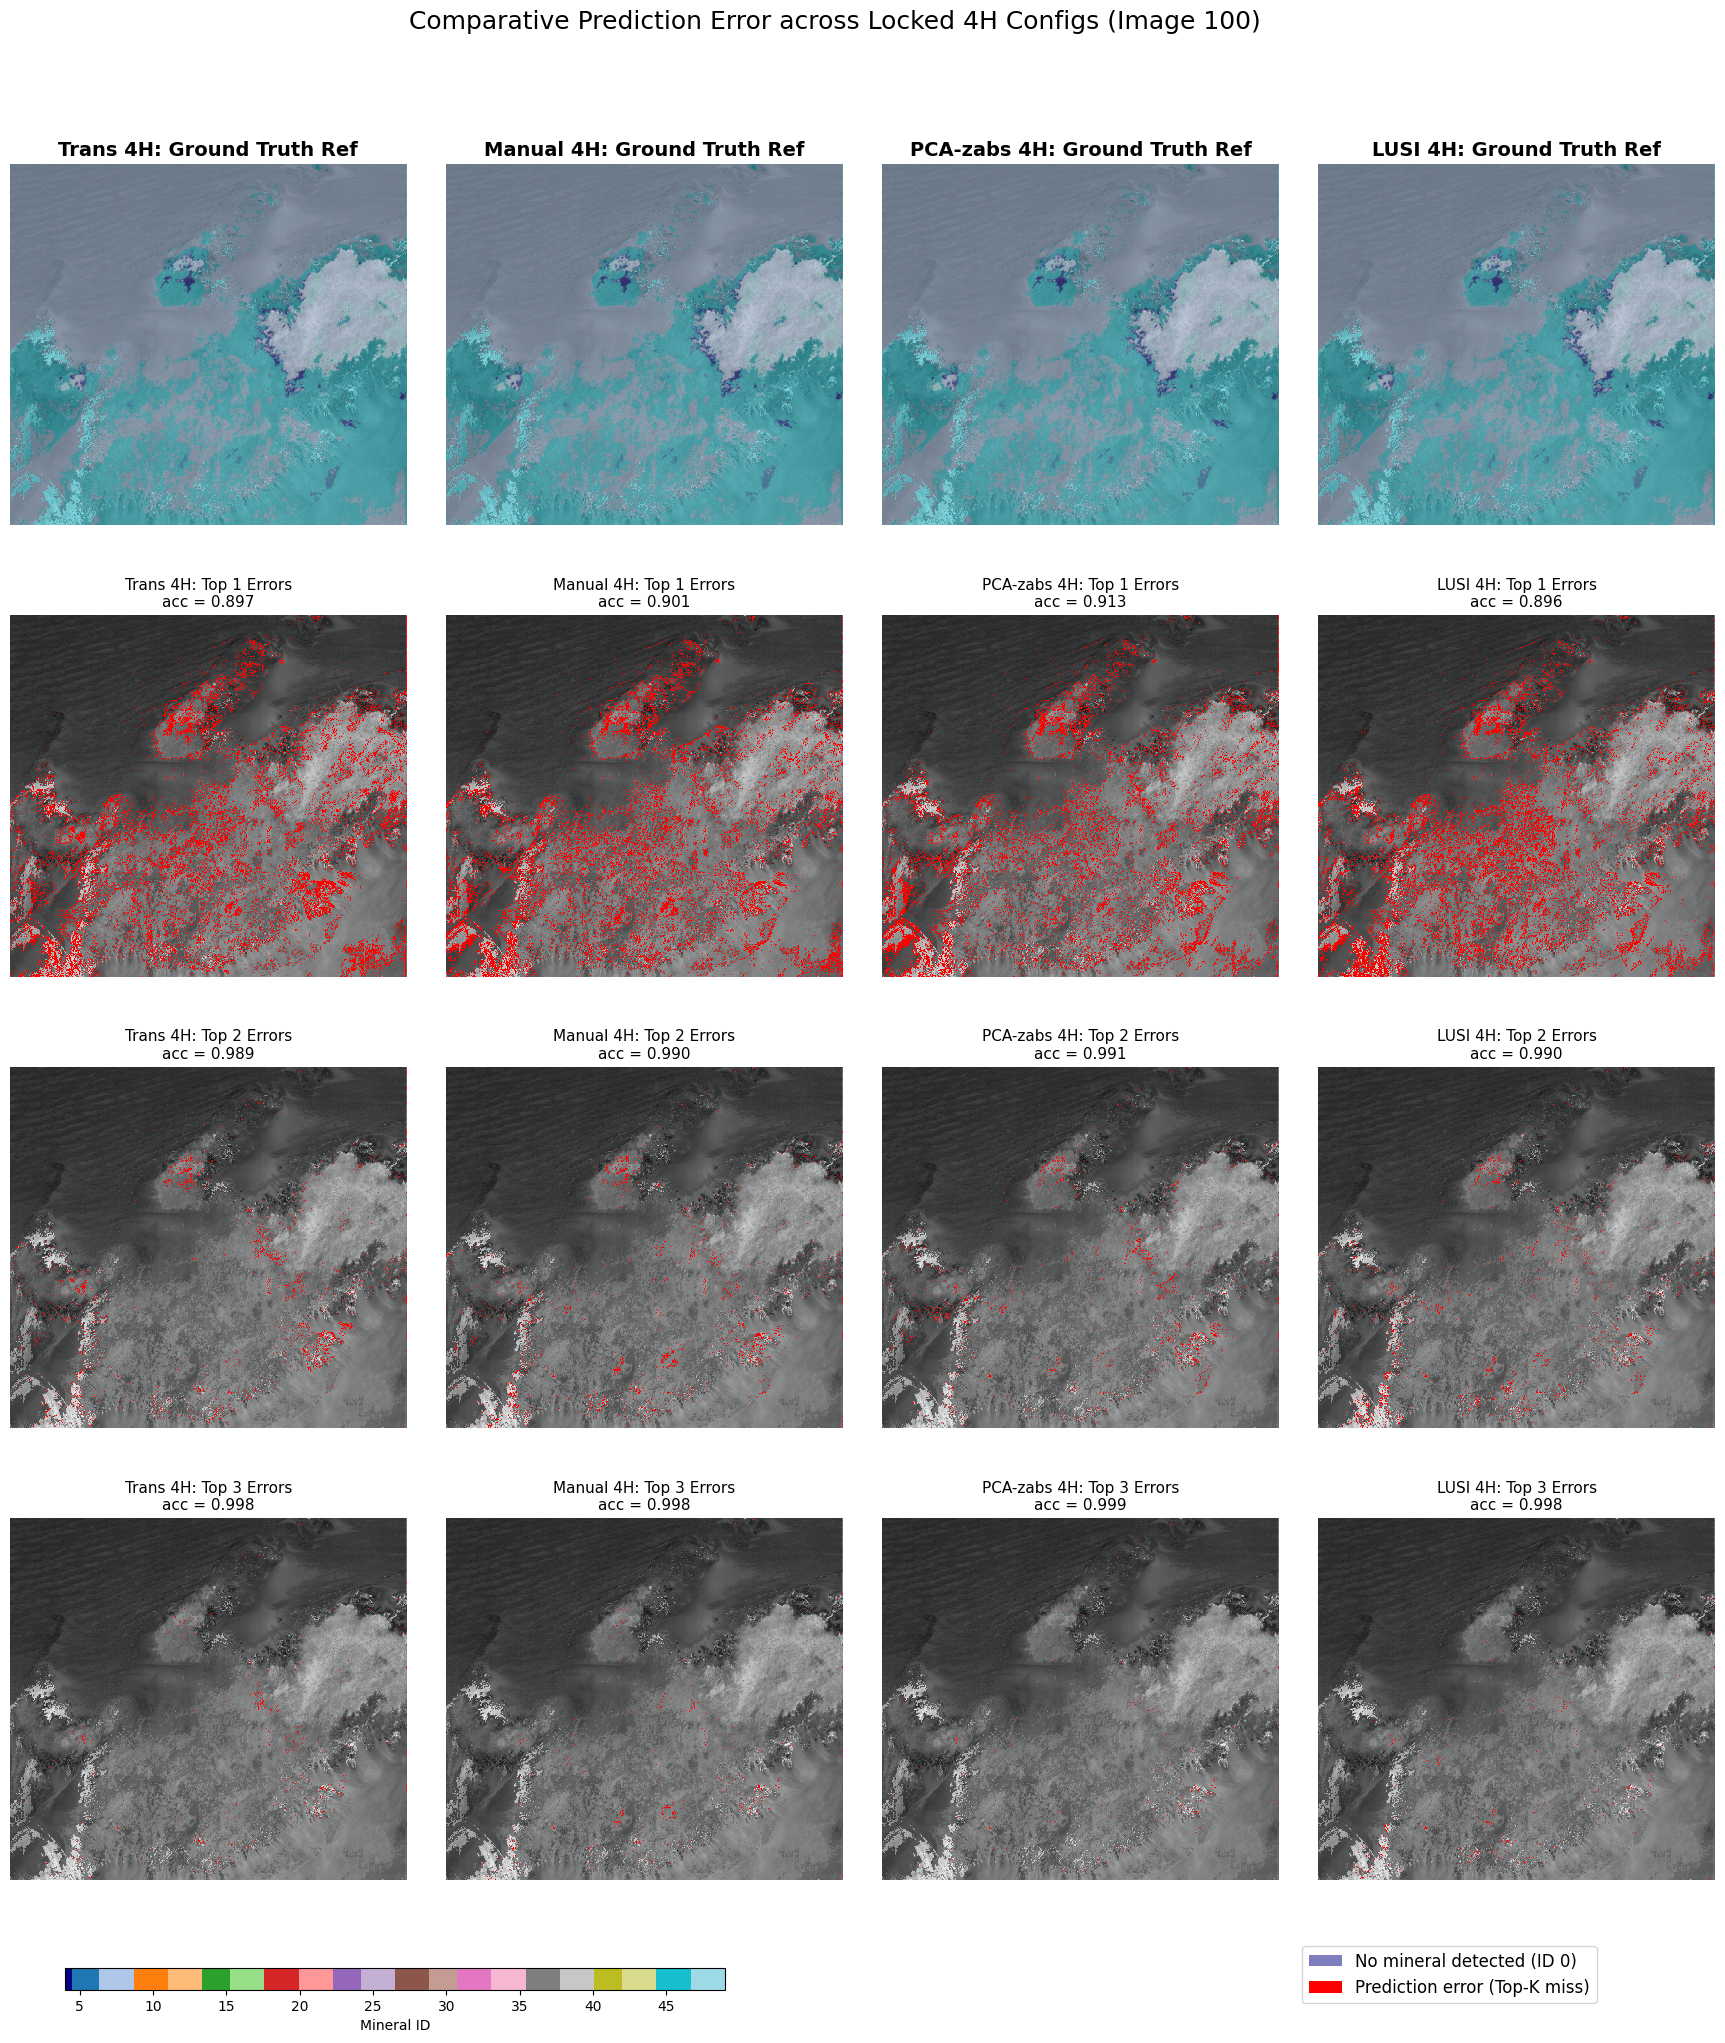
\includegraphics[width=\textwidth]{granule_error_grid_image50.png}
\caption{Spatial distribution of prediction errors on Image~50 across the four locked $H = 4$ configurations of Table~\ref{tab:ablation}. \textbf{Columns:} transformer baseline, manual prior, PCA-curated prior, LUSI. \textbf{Rows:} ground-truth Group~1 mineral ID (top, navy = no-mineral); top-1 errors (red where the highest-probability prediction is incorrect); top-2 errors (red where neither the top-1 nor the top-2 prediction is correct); top-3 errors (red where all three are wrong). Per-panel accuracies are annotated above each subplot. The top-1 ranking on this granule is PCA-curated (0.847) $>$ Manual (0.836) $>$ Trans (0.827) $>$ LUSI (0.808), matching the validation-pool ordering. The top-3 row is visually near-saturated ($0.987$--$0.996$) --- once the answer is allowed to be among the top three predictions, all four configurations recover the correct class on essentially every mineral pixel. Errors concentrate in the same spatial region across all four configurations, indicating a region-level rather than configuration-level failure mode. The full four-granule, four-metric table is reported in the dissertation.}
\label{fig:granule_error_grid}
\end{figure}

Cross-region granule deployment is reported in Table~\ref{tab:crossscene} across 20 mineral-populated SW US granules (each with $\geq 20\%$ Group-1 mineral pixels). The cross-region winning configuration is head-count-dependent: at $H = 4$ the sharp manual prior leads (SW top-1 $= 0.724$), while at $H = 8$ the diffuse PCA-curated prior leads (SW top-1 $= 0.705$). The reversal mirrors the in-distribution sharp-vs-diffuse pattern of Table~\ref{tab:ablation}: narrow Gaussian bumps over-constrain attention at saturated capacity, while PCA-curated's diffuse loadings ($\sim$$220$ of $285$ bands) anchor better when more heads are available. LUSI is last or next-to-last on both top-1 and top-3 at both head counts, providing no consistent cross-region advantage.

\section{Discussion and conclusions}
\label{sec:conclusions}

%% ====================================================================
%% REFERENCES
%% ====================================================================
\bibliographystyle{elsarticle-num}
\bibliography{references}

\end{document}
